\documentclass[11pt,a4paper]{article}

\usepackage{fontspec}
\usepackage{unicode-math}
\setmainfont{Latin Modern Roman}
\setsansfont{Latin Modern Sans}
\setmonofont{DejaVu Sans Mono}[Scale=0.82]
\setmathfont{Latin Modern Math}
\usepackage[margin=2.6cm]{geometry}
\usepackage{amsmath,amsthm,mathtools}
\usepackage{graphicx}
\usepackage{booktabs}
\usepackage{longtable}
\usepackage{enumitem}
\usepackage{xcolor}
\usepackage[colorlinks=true,linkcolor=blue!50!black,citecolor=blue!50!black,urlcolor=blue!50!black]{hyperref}
\usepackage{tikz}
\usetikzlibrary{arrows.meta,positioning,fit,backgrounds,calc,decorations.pathreplacing}
\usepackage{listings}
\usepackage{microtype}

\lstdefinestyle{lean}{
  language=ML,
  basicstyle=\ttfamily\footnotesize,
  keywordstyle=\color{blue!60!black}\bfseries,
  commentstyle=\color{green!40!black}\itshape,
  stringstyle=\color{red!50!black},
  showstringspaces=false,
  breaklines=true,
  columns=fullflexible,
  frame=single,
  framerule=0.3pt,
  rulecolor=\color{black!30},
  xleftmargin=1em,
}
\lstset{style=lean}

\theoremstyle{plain}
\newtheorem{theorem}{Theorem}[section]
\newtheorem{proposition}[theorem]{Proposition}
\newtheorem{lemma}[theorem]{Lemma}
\newtheorem{corollary}[theorem]{Corollary}
\theoremstyle{definition}
\newtheorem{definition}[theorem]{Definition}
\newtheorem{example}[theorem]{Example}
\newtheorem{remark}[theorem]{Remark}
\newtheorem{conjecture}[theorem]{Conjecture}

\newcommand{\R}{\mathbb{R}}
\newcommand{\T}{\mathbb{T}}
\newcommand{\N}{\mathbb{N}}
\newcommand{\Z}{\mathbb{Z}}
\newcommand{\C}{\mathbb{C}}
\newcommand{\eps}{\varepsilon}
\newcommand{\dd}{\,\mathrm{d}}
\newcommand{\Ltwo}{L^2}
\newcommand{\Linf}{L^\infty}
\newcommand{\Hs}{H^s}
\newcommand{\Lp}{L^p}
\newcommand{\Cont}{C^\infty}
\newcommand{\Contc}{C^\infty_c}
\newcommand{\Conts}{C^\infty_\sigma}
\newcommand{\lean}[1]{\texttt{\detokenize{#1}}}
\newcommand{\file}[1]{\texttt{\detokenize{#1}}}
\newcommand{\norm}[1]{\left\lVert #1 \right\rVert}
\newcommand{\abs}[1]{\left\lvert #1 \right\rvert}
\newcommand{\ip}[2]{\left\langle #1, #2 \right\rangle}
\newcommand{\TauCeti}{\textsf{TauCeti}}
\newcommand{\Mathlib}{\textsf{Mathlib}}
\newcommand{\Lean}{\textsf{Lean}}

\title{\bfseries Finite-Time Blowup for the\\ Three-Dimensional Navier--Stokes and Euler Equations\\[4pt]
\large A Complete Machine-Checked Formalization, and Its Migration to\\
Current \Mathlib{} and \TauCeti{}}
\author{Open Math Model Project\thanks{Formalization originally produced by OpenAI;
this report documents the statement audit, library migration and verification of the
repository \texttt{NavierStokesAndEuler}.}}
\date{\today}

\begin{document}
\maketitle

\begin{abstract}
We report on a complete, machine-checked formalization of two recent results on
singularity formation in three-dimensional incompressible fluid mechanics: the
construction, for every positive viscosity, of a smooth compactly supported force and
zero initial data whose Navier--Stokes solution develops unbounded velocity in finite
time while its kinetic energy stays uniformly bounded (Clay alternatives \textbf{(C)}
and \textbf{(D)} of the Millennium Prize problem statement), and the construction of a
smooth compactly supported divergence-free initial velocity whose solution of the
unforced incompressible Euler equations breaks down in finite time, with unbounded
$C^1$ norm and divergent time integral of the vorticity $L^\infty$ norm. The
formalization comprises \textbf{2{,}588 Lean~4 files} and \textbf{541{,}000 lines} of
proof text, with \textbf{30{,}630} theorem and lemma declarations and no gaps in the
proof libraries; every headline result depends only on the three standard axioms
\texttt{propext}, \texttt{Classical.choice} and \texttt{Quot.sound}. Beyond stating the
results, the paper has two purposes. First, it gives a reader's guide to what was
actually formalized: the statement engineering that pins each analytic claim to its
literal $\R^3$ or $\T^3$ meaning, the module architecture of the two developments, and
the way the oscillatory constructions of the source papers---similarity coordinates,
dyadic charts, pulse and packet families, correction cycles and summation with
shrinking cuts---are represented as Lean objects. Second, it reports an engineering
migration of the repository from its original pin (Lean \texttt{v4.34.0-rc2}) to the
current library generation (Lean \texttt{v4.36.0-rc1}, \Mathlib{} at \texttt{2cabef97},
\TauCeti{} at \texttt{b8cbc77}), with the API breakage that this caused classified and
repaired where encountered, a catalogue of which project-local analysis gadgets a
library such as \TauCeti{} can and cannot replace, a measurement of how much of the code
duplicates the libraries (little, and concentrated in one layer of eighteen files) against
how much duplicates itself, and an assessment of what a migration of this kind costs at this
scale. Worked examples---the core's energy budget, the exponent ledger, the viscosity
rescaling term by term, and the packet amplitudes---are given with explicit numbers.

\end{abstract}

\tableofcontents
\newpage

\section{Introduction}
\label{sec:intro}

\subsection{The problem}

The Clay Mathematics Institute's formulation of the Navier--Stokes problem
\cite{clay} asks, among other things, for a decision on four alternatives. Two of them are
blowup statements: \textbf{(C)} that there exist smooth compactly supported data and a
smooth force on $\R^3$ for which no global smooth solution with uniformly bounded kinetic
energy exists, and \textbf{(D)} the same on the torus $\R^3/\Z^3$. Two recent papers of
OpenAI \cite{ns-paper,euler-paper} prove both, and prove in addition that the
\emph{unforced} three-dimensional Euler equations admit a smooth compactly supported
initial velocity whose solution develops a singularity in finite time. Those three
theorems are the subject of this paper.

The mechanisms are different and both are intricate. The Navier--Stokes construction builds
a self-similar vortex whose core contracts anisotropically towards a point as $t\uparrow1$,
whose azimuthal and axial velocities grow like $\tau^{-1/2-h}$ with $\tau=1-t$, and whose
residual is not zero but is concentrated in an annulus where it is realised, exactly, as
the divergence of a tangential stress. Two families of spatially oscillatory pulses are
placed in the annulus; their averaged quadratic fluxes supply that stress, and a fixed
cycle of four corrections then improves the decay of the residual until it is flat---all
Cartesian derivatives vanish to every order at the singular point---at which point it can be
absorbed into a smooth compactly supported force. The energy of the whole field tends to
zero at the singular time, which is what makes the result a statement about
\emph{non-existence} of a bounded-energy continuation. The Euler construction is an
iteration on exact solutions: a localized oscillation (a \emph{packet}) is added to a
smooth flow, its gradient is amplified by the shear of the flow it sits in, and the
amplified gradient becomes the shear that amplifies the next packet; the initial data
converge in every Sobolev norm while the gradients at the target times diverge.

\subsection{What has been done}

Both results, and both Navier--Stokes alternatives, have been formalized in Lean~4
\cite{lean} on top of \Mathlib{} \cite{mathlib}. The development reported here consists of
2{,}500 files and 542{,}072 lines of Lean source containing 30{,}630 theorem and lemma
declarations; two reductions along the way, the removal of unreachable modules and the
removal of unused lemmas, took it down from 2{,}659 files and 643{,}986 lines with 36{,}825
declarations (Section~\ref{sec:cleanup}, Section~\ref{sec:unused}). It has no \lean{sorry} in its proof libraries and no axioms beyond
\lean{propext}, \lean{Classical.choice} and \lean{Quot.sound} (Section~\ref{sec:verification}).
The headline statements are the reference statements: the Euler definitions and both
challenge modules are adapted from the Formal Conjectures formalization
\cite{formalconj} of the Millennium problem, not paraphrased.

\subsection{What this paper does}

A development of this size is not useful if the only thing that can be said about it is
that it compiles. The paper therefore has three aims.

\emph{A reader's guide.} Sections~\ref{sec:results} and~\ref{sec:scheme} state what is
actually proved, with exact declaration names, and describe the construction at the level
of detail the Lean development encodes---including the objects that a paper leaves implicit
and a formalization cannot: the dyadic charts, the auxiliary tori used to separate
oscillating pulses, the reserved logarithmic patches, the exponent ledger. A reader who
wants to know whether a specific estimate of the source paper was really formalized, and
where, should be able to find out.

\emph{An architecture report.} Section~\ref{sec:architecture} describes how the development
is organised---three layers (statements, infrastructure, construction), an unusually flat
import graph, a naming discipline that follows the mathematics---and reports measurements:
file sizes, import-graph depth, the 74 modules that no entry point reaches.

\emph{A verification and migration record.} Section~\ref{sec:verification} reports the trust
base and the statement audit. Section~\ref{sec:libraries} documents the migration of the
repository from Lean \texttt{v4.34.0-rc2} to \texttt{v4.36.0-rc1}, from its original
\Mathlib{} pin to \Mathlib{} \texttt{2cabef97}, and to the downstream analysis library
\TauCeti{} \cite{tauceti}, together with a catalogue of what the migration broke and why.
Section~\ref{sec:assessment} is an assessment, including what the formalization does
\emph{not} establish.

\subsection{Related work}

Machine-checked formalizations of research-level mathematics have moved in a decade from
individual theorems (the odd order theorem, the Kepler conjecture \cite{flyspeck}) to
whole areas: the sphere eversion, the liquid tensor experiment, the polynomial Freiman--Ruzsa
conjecture, Fermat's Last Theorem for regular primes. What distinguishes the present
development is that its objects are \emph{partial differential equations} and that its
statements are \emph{non-existence} statements obtained by explicit construction: every
field appearing in the headline theorems is built, not postulated, and the properties are
proved of the constructed object. The closest formal neighbours are the Formal Conjectures
statements \cite{formalconj}, which supply the reference formulations used here but no
proofs, and the general \Mathlib{} analysis library, which supplies most of the
point-set, measure-theoretic and functional-analytic infrastructure but has, at the pinned
version, only a predicate-level theory of Sobolev spaces.

\subsection{Organisation}

Section~\ref{sec:results} states the theorems. Section~\ref{sec:scheme} describes the two
constructions and their formal counterparts. Section~\ref{sec:architecture} is the
architecture report. Section~\ref{sec:verification} is the verification report.
Section~\ref{sec:libraries} is the migration report, including a measurement of how much
of the code duplicates the libraries and where the real duplication lies.
Section~\ref{sec:examples} works four computations through explicitly---the energy budget of
the core, the exponent ledger, the viscosity rescaling and the packet amplitudes---and gives
two code-level examples of the migration. Section~\ref{sec:assessment} assesses.
The appendices reproduce the headline statements verbatim, index the modules a reader
should open first, and record the migration's changes to the repository.

\section{The formalized statements}
\label{sec:results}

This section states exactly what the repository proves. Every statement below is a
transcription of a Lean declaration; we give the declaration name so that a reader can
check the transcription against the source. Throughout, $u$ denotes a velocity field
and $p$ a pressure field on spacetime; the Lean encoding uses
\[
  \texttt{Space} := \R^3 = \texttt{EuclideanSpace}\ \R\ (\texttt{Fin}\ 3),
  \qquad
  \texttt{SpaceTime} := \R \times \R^3,
\]
with time as the \emph{first} coordinate. Vector-valued fields are functions
$\R\times\R^3 \to \R^3$ and are total; every regularity, support and integrability
condition that a paper would leave implicit is an explicit hypothesis.

\subsection{The differential operators}
\label{sec:operators}

The repository does not use a bundled ``solution'' structure with an opaque equation.
All operators are defined from the Fr\'echet derivative, in
\file{NavierStokes/ProblemStatement.lean}:
\begin{align*}
  \partial_t u(t,x) &:= \mathrm{d}f(\lambda s.\, u(s,x))(t)(1), \\
  (u\cdot\nabla)u\,(t,x) &:= \mathrm{d}f(\lambda y.\, u(t,y))(x)\bigl(u(t,x)\bigr), \\
  \nabla\cdot u\,(t,x) &:= \textstyle\sum_{i<3} \mathrm{d}f(\lambda y.\,u(t,y))(x)(e_i)_i, \\
  \Delta u\,(t,x) &:= \textstyle\sum_{i<3} \mathrm{d}f\bigl(\lambda y.\, \mathrm{d}f(\lambda z.\,u(t,z))(y)(e_i)\bigr)(x)(e_i), \\
  \nabla p\,(t,x) &:= \textstyle\sum_{i<3} \mathrm{d}f(\lambda y.\,p(t,y))(x)(e_i)\, e_i,
\end{align*}
where $e_0,e_1,e_2$ are \lean{coordinateVector i}, the unit coordinate vectors. The
residual at viscosity $\nu$ is then
\begin{equation}
  \mathcal{R}_\nu(u,p) \;=\; \partial_t u + (u\cdot\nabla)u - \nu\,\Delta u + \nabla p,
  \label{eq:residual}
\end{equation}
and the equation is imposed \emph{pointwise at interior times} $0<t<1$ (respectively
$t>0$), with the initial condition imposed separately at $t=0$. This distinction
matters: no extension of $u$ to negative times is differentiated at the boundary, and
the differentiability hypothesis at time zero is taken relative to the physical
half-domain $\{0\le t<1\}\times\R^3$.

\subsection{Blowup for forced Navier--Stokes on $\R^3$}
\label{sec:r3}

\begin{theorem}[Whole-space breakdown; \lean{NavierStokesR3.ProblemStatement.breakdownStatement},
  proved as \lean{NavierStokesR3.theorem_1_1} in \file{NavierStokes/R3/Theorem.lean}]
\label{thm:ns-r3}
For every $\nu>0$ there exist a velocity field $u$, a pressure $p$, a force $f$ and a
compact set $K\subseteq\R^3$ such that:
\begin{enumerate}[label=\textup{(i\arabic*)}]
  \item $u$ and $p$ are $C^\infty$ on $\{0\le t<1\}\times\R^3$, and $f$ is
        $C^\infty$ on $\{t\ge 0\}\times\R^3$;
  \item $f$ has compact support in spacetime, contained in $\{t>0\}$;
  \item $u(\cdot,t)$ and $p(\cdot,t)$ are supported in the same fixed compact $K$ for
        every $0\le t<1$;
  \item $u(0,x)=0$ for all $x$;
  \item $\nabla\cdot u(t,x)=0$ for $0\le t<1$;
  \item $\mathcal{R}_\nu(u,p)(t,x)=f(t,x)$ for $0<t<1$;
  \item there is $E\ge 0$ with $\int_{\R^3}|u(t,x)|^2\dd x \le 2E$ for every
        $0\le t<1$ (and each such slice is integrable);
  \item for every $M$ and every $\delta>0$ there are $t,x$ with $0<t<1$,
        $1-\delta<t$ and $|u(t,x)|>M$;
  \item there is \emph{no} velocity field $v$ and pressure $P$, $C^\infty$ on
        $\{t\ge 0\}\times\R^3$ with $v(0,\cdot)=0$ and $\nabla\cdot v=0$, solving
        $\mathcal{R}_\nu(v,P)=f$ for all $t>0$ and with uniformly bounded kinetic
        energy $\sup_{t\ge0}\int|v(t,x)|^2\dd x<\infty$.
\end{enumerate}
\end{theorem}

Points (i)--(vi) are the fields \lean{CandidateProperties} of
\file{NavierStokes/R3/ProblemStatement.lean}; (vii) and (viii) are the components
\lean{energy_bounded} and \lean{speed_unbounded} of the same structure; (ix) is
\lean{¬ Nonempty (GlobalFiniteEnergySolution ν f)}. The competitor in (ix) is
deliberately given \emph{no} support, periodicity, pressure-growth or energy-inequality
assumption beyond smoothness, the equation, incompressibility, the zero datum and a
uniform bound on the kinetic energy: it is exactly the class in which the theorem
claims non-existence. The energy in (vii) is required at every time of the half-open
interval $[0,1)$, including $t=0$, which is why square integrability is part of the
statement rather than an afterthought.

\begin{remark}[Two refinements carried by the formal proof]
\label{rem:r3-refine}
The repository proves two strengthenings that are not visible in the statement of
Theorem~\ref{thm:ns-r3}. First, \lean{theorem_1_1_with_initial_rest} produces the same
witnesses with $u(t,x)=p(t,x)=0$ for all $|t|\le 3/8$: the flow is at rest for a full
symmetric time interval around zero, so the force is switched on smoothly out of the
zero state. Second, \lean{theorem_1_1_with_dissipation} proves the energy balance satisfied by the
same constructed fields: with
$\mathrm{diss}(t)=\sum_{i}\int_{\R^3}|\partial_i u(t,x)|^2\dd x$ and
$F(T)=\int_0^T\|f(t)\|_{L^2}\dd t$, it shows that $f$ is interval-integrable,
$\mathrm{diss}$ is integrable on $[0,1)$, and for every $T\in[0,1)$
\[
  \|u(T)\|_{L^2}^2 + 2\nu\int_0^T \mathrm{diss}(t)\dd t \;\le\; F(T)^2 ,
\]
so the constructed solution satisfies the energy inequality with equality of constants and,
in particular, has finite total dissipation before the singular time. This is the
formal counterpart of Lemma~10.4 of the source paper, and it is a statement about the
\emph{localized} fields, obtained from the equation rather than from the construction.
\end{remark}

\subsection{Blowup on the torus}
\label{sec:torus}

The torus is \emph{not} modelled by a quotient type. It is modelled by
$\Z^3$-periodic functions on $\R^3$: a field $g$ satisfies \lean{UnitSpatialPeriodsOn}
on a time set $T$ if $g(t,x+e_i)=g(t,x)$ for all $t\in T$, $x\in\R^3$ and
$i\in\{0,1,2\}$. Support statements are then intersections with the closed fundamental
cube, so that a nonzero periodic lift is never claimed to have compact support on
$\R^3$; that would be false.

\begin{theorem}[Periodic breakdown; \lean{NavierStokes.PeriodicPaper.breakdownStatement},
  proved as \lean{NavierStokes.PeriodicPaper.periodic_corollary} in
  \file{NavierStokes/PeriodicPaperTheorem.lean}]
\label{thm:ns-torus}
For every $\nu>0$ there exist $u,p,f$ and a compact $K$ contained in the interior of the
fundamental cube such that:
\begin{enumerate}[label=\textup{(i\arabic*)}]
  \item $u,p$ are $C^\infty$ on $\{0\le t<1\}\times\R^3$ and $f$ is $C^\infty$ on
        $\{t\ge0\}\times\R^3$;
  \item $u(\cdot,t)$ and $p(\cdot,t)$ are unit-periodic in space for $0\le t<1$, and
        $f$ is unit-periodic for $t\ge0$;
  \item $u(\cdot,t)$ and $p(\cdot,t)$ have support meeting the closed fundamental cube
        in $K$, and $f$ vanishes identically for $t\le 0$ and for all $t\ge T_0$ for
        some $T_0<\infty$;
  \item $u(0,\cdot)=0$, $\nabla\cdot u=0$ for $0\le t<1$, and
        $\mathcal{R}_\nu(u,p)=f$ for $0<t<1$;
  \item for every $M$ and $\delta>0$ there are $t,x$ with $0<t<1$, $1-\delta<t$ and
        $|u(t,x)|>M$;
  \item there is no globally defined, spatially periodic, $C^\infty$ solution of
        $\mathcal{R}_\nu(v,P)=f$ with $v(0,\cdot)=0$ and $\nabla\cdot v=0$.
\end{enumerate}
\end{theorem}

The proof of Theorem~\ref{thm:ns-torus} is not a re-run of the whole construction.
\lean{periodic_corollary} takes the $\R^3$ witnesses of
Theorem~\ref{thm:ns-r3}, compresses them by an affine parabolic scaling to bring their
support into the fundamental domain, and then reads the resulting fields as periodic
lifts; the ``periodization'' of the equations is the content of
\file{NavierStokes/PeriodizePDE.lean}. The scaling is a parabolic rather than a plain
similarity precisely because the equation is not scale invariant at fixed viscosity; the
clock is preserved, so the singular time stays exactly one.

\subsection{Blowup for the unforced Euler equation}
\label{sec:euler}

The Euler development is built on the definitions of the \emph{Formal Conjectures}
project, adapted verbatim in \file{Euler/SolutionDefinitions.lean}, with velocity and
pressure taking position \emph{before} time. The reference development supplies two
distinct conclusions: the Beale--Kato--Majda-flavoured non-continuation statement, and a
quantitative statement that exhibits the maximal lifespan as a genuine object with the
blowup properties.

\begin{theorem}[Euler non-continuation; \lean{Euler.euler\_breakdown\_R3} in
  \file{Euler/Solution.lean}]
\label{thm:euler-bkm}
There is $u_0\in C^\infty(\R^3;\R^3)$ with $\nabla\cdot u_0=0$, whose every spatial
derivative decays faster than any polynomial, and such that there is no pair $(v,p)$
of $C^\infty$ fields on $\{t\ge0\}$ solving
$\partial_t v+(v\cdot\nabla)v=-\nabla p$, $\nabla\cdot v=0$, $v(\cdot,0)=u_0$, with
finite uniformly bounded energy.
\end{theorem}

\begin{theorem}[Quantitative Euler singularity;
  \lean{Euler.exists\_compact\_smooth\_euler\_singularity} in \file{Euler/Solution.lean}]
\label{thm:euler-quant}
There are $u_0\in C^\infty(\R^3;\R^3)$ with $\nabla\cdot u_0=0$, $u_0\ne0$,
$\operatorname{supp}u_0$ compact, and $T_*\in(0,1]$ such that
\begin{enumerate}[label=\textup{(i\arabic*)}]
  \item for every $T>0$, a smooth solution on $[0,T]$ with datum $u_0$ exists if and only
        if $T<T_*$;
  \item the velocity stays bounded in $L^2$ uniformly on $[0,T_*)$;
  \item for every $T<T_*$, $\sup_{0\le t\le T}\|v(t)\|_{C^1}<\infty$ and
        $\int_0^T\|\operatorname{curl}v(t)\|_\infty\dd t<\infty$, while
        \[
          \limsup_{t\uparrow T_*}\|\nabla v(t)\|_\infty=\infty,
          \qquad
          \int_0^{T_*}\|\operatorname{curl} v(t)\|_\infty\dd t=\infty .
        \]
\end{enumerate}
\end{theorem}

Theorem~\ref{thm:euler-quant}, in the form \lean{exists_compact_smooth_euler_singularity}
of \file{Euler/EulerSingularity.lean}, is stated in terms of an explicit structure
\lean{FiniteLifespan A} which carries the maximal solution: a family of smooth solutions
on $[0,T]$ for $T<T_*$, their compatibility, and the assertion that no solution exists on
$[0,T]$ for $T\ge T_*$. The point of this formulation is that ``$T_*$ is the maximal
lifespan'' is a \emph{proved property of a constructed object}, not a hypothesis: the
bulk of the Euler development is a construction of that object
(\file{Euler/EulerProof.lean} is the 20{,}755-line core) together with the identification
of its norms with the pointwise suprema of the actual velocity, derivative and curl.

\begin{remark}[Statement fidelity]
\label{rem:fidelity}
The definitions of \file{Euler/SolutionDefinitions.lean} and
\file{ComparatorChallenges/Euler.lean} are copied from the Formal Conjectures
formalization of the Millennium problem statement and are not modified. Consequently the
Euler results are proved for the reference statement itself, and not for a convenient
variant of it; the same holds for the Navier--Stokes alternatives \textbf{(C)} and
\textbf{(D)}, whose reference definitions are imported by
\file{NavierStokes/ComparatorSolution.lean}. Section~\ref{sec:verification} reports the
axiom audit that makes this claim checkable.
\end{remark}

\section{The blowup scheme, and what had to be formalized}
\label{sec:scheme}

A formalization paper is only useful if a reader can see what mathematics the machine was
asked to check. This section describes the two constructions at the level of detail that
the Lean development actually encodes, and names for each ingredient the module in which
it lives. We do not reproduce the analytic proofs; we describe their architecture and
flag the places where a paper argument had to become a Lean object.

\subsection{Navier--Stokes: the shape of the construction}
\label{sec:ns-shape}

The solution is built so that the singularity forms at the origin at time $t=1$ from the
zero datum, with the force switched on after a full initial rest interval
($|t|\le 3/8$, Remark~\ref{rem:r3-refine}). Write $\tau=1-t$ and let $h\in(0,1/100)$ be a
fixed small exponent. The construction distinguishes four regions, at time $t$:

\begin{center}
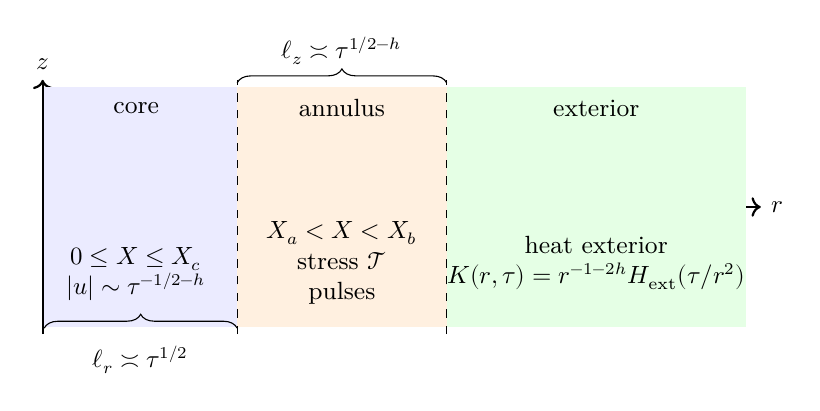
\begin{tikzpicture}[scale=0.95,every node/.style={font=\small}]
  % axis
  \draw[->,thick] (0,0) -- (9.6,0) node[right] {$r$};
  \draw[->,thick] (0,-1.7) -- (0,1.7) node[above] {$z$};
  % regions as vertical bands
  \fill[blue!8]  (0.02,-1.6) rectangle (2.6,1.6);
  \fill[orange!12] (2.6,-1.6) rectangle (5.4,1.6);
  \fill[green!10] (5.4,-1.6) rectangle (9.4,1.6);
  \draw[dashed] (2.6,-1.7) -- (2.6,1.7);
  \draw[dashed] (5.4,-1.7) -- (5.4,1.7);
  \node at (1.25,1.32) {core};
  \node at (4.0,1.32) {annulus};
  \node at (7.4,1.32) {exterior};
  \node[align=center] at (1.25,-0.9) {$0\le X\le X_c$\\$|u|\sim \tau^{-1/2-h}$};
  \node[align=center] at (4.0,-0.75) {$X_a<X<X_b$\\stress $\mathcal{T}$\\pulses};
  \node[align=center] at (7.4,-0.75) {heat exterior\\$K(r,\tau)=r^{-1-2h}H_{\mathrm{ext}}(\tau/r^2)$};
  \draw[decorate,decoration={brace,amplitude=5pt}] (0.02,-1.62) -- (2.6,-1.62) node[midway,below=3pt] {$\ell_r\asymp\tau^{1/2}$};
  \draw[decorate,decoration={brace,amplitude=5pt}] (2.6,1.66) -- (5.4,1.66) node[midway,above=3pt] {$\ell_z\asymp\tau^{1/2-h}$};
\end{tikzpicture}
\end{center}

\begin{enumerate}[label=(\roman*)]
  \item \textbf{Core.} An axisymmetric field whose azimuthal and axial components grow like
        $\tau^{-1/2-h}$ while the radial component grows only like $\tau^{-1/2}$. The core
        is slender: radial scale $\tau^{1/2}$, axial scale $\tau^{1/2-h}$. It solves its
        own leading profile equations exactly, by construction: the profiles $E,U,V_0,\Pi$
        are chosen to satisfy the leading azimuthal and axial balances with radial
        viscosity retained and axial viscosity discarded.
  \item \textbf{Annulus.} Where the core is joined to the exterior, the joining error is
        not smooth in $\tau$. It is written, exactly, as the divergence of a tangential
        stress,
        \[
          R^{(0)}_\theta = -\Bigl(\partial_r+\tfrac2r\Bigr)T_{r\theta},
          \qquad
          R^{(0)}_z = -\Bigl(\partial_r+\tfrac1r\Bigr)T_{rz},
        \]
        supported in an annulus $X_a<X<X_b$ in the similarity variable $X=r^2/2q$.
  \item \textbf{Pulses.} Two families of spatially oscillatory, divergence-free velocities
        are placed in the annulus. Their averaged quadratic fluxes
        $\langle w_r w_\theta\rangle,\langle w_r w_z\rangle$ are made equal to
        $T_{r\theta},T_{rz}$. The families are chosen so that the target stress lies in the
        \emph{interior} of the cone they generate, which is what makes the amplitudes
        positive and the construction stable under perturbation.
  \item \textbf{Exterior.} A purely azimuthal field $K(r,\tau)e_\theta$ solving the radial
        heat equation for the swirl exactly, so that its residual vanishes identically and
        no force is needed there. Its decay rate $r^{-1-2h}$ is what makes the kinetic
        energy of the whole field finite.
\end{enumerate}

The residual of the background plus leading pulses is then not zero but \emph{flat}: every
Cartesian space--time derivative is $O(q^N)$ for every $N$, with $q$ the concentration
scale. Flatness is converted into a smooth force by the localization and extension step.
The single most important structural fact is that the whole construction is a
\emph{finite-stage} object with an \emph{infinite} limit taken at the very end, and that
the limit is taken on vector potentials, not on velocities.

\subsection{The correction cycle}
\label{sec:correction}

Starting from the background plus leading waves, the construction repeats a fixed cycle of
four operations. Writing $u^{[j]},p^{[j]}$ for the fields after $j$ cycles,
\begin{equation}
  u^{[j+1]} = u^{[j]} + \delta u_j,
  \qquad
  p^{[j+1]} = p^{[j]} + \delta p_j,
\end{equation}
the residual changes by the exact identity
\begin{equation}
  \mathcal{R}(u^{[j+1]},p^{[j+1]}) = \mathcal{R}(u^{[j]},p^{[j]})
   + L_{u^{[j]}}(\delta u_j,\delta p_j) + \nabla\cdot(\delta u_j\otimes\delta u_j),
  \label{eq:increment}
\end{equation}
where $L_v$ is the linearization of $\mathcal{R}$ at $v$. The four operations are: solve the
inhomogeneous amplitude equations on the supported angular modes; add signed amplitude
increments whose cross-covariance with the leading pulses supplies a prescribed correction
to the mean stress; correct the angularly averaged residual by inverting the auxiliary-time
derivative; and solve five radial moment equations that keep the pressure and the two
tangential momentum fluxes consistent across the annulus. Each cycle improves a
\emph{residual exponent} $\sigma_j$:
\begin{equation}
  \sigma_0=\tfrac15,\qquad \sigma_{j+1}=\sigma_j+\tfrac1{10},
  \qquad \sigma_j \longrightarrow \infty .
  \label{eq:sigma}
\end{equation}
The exponent arithmetic---which powers of $q$, $S_*=\ell^2$ and the logarithmic edge
weights survive each of the four operations---is isolated in
\file{NavierStokes/ExponentLedger.lean}, a file with no analysis in it at all: it checks the
bookkeeping of \eqref{eq:sigma} against the manuscript's Proposition~10.3, conditionally on
the estimates being valid. This separation is one of the more useful things the
formalization does: the part of the argument that is pure arithmetic is a Lean file about
real numbers, and the part that is analysis is a Lean file about PDEs, and neither can hide
a mistake in the other.

\subsection{Summation, localization and the force}
\label{sec:summation}

The corrections are summed with cutoffs on their \emph{vector potentials}: at stage $j$ one
multiplies the potential $A_j$ and the pressure increment $p_j$ by a cutoff that equals one
on a neighbourhood of the singular point and whose support shrinks with $j$, and then takes
the curl. Taking the curl after multiplication is what keeps incompressibility exact at
every stage. The cutoff losses are controlled because the stage-$j$ estimates lose a power
of $q$ that depends on the derivative order but not on $j$.

After summation one has a local pair $(u_{\mathrm{loc}},p_{\mathrm{loc}})$ on
$\{\tau>0,\ q<q_*\}$ with a potential representation
\begin{equation}
  u_{\mathrm{loc}} = \nabla\times A + B\,e_\theta,
  \label{eq:potential}
\end{equation}
in which both terms are separately divergence-free and both are smooth in Cartesian
coordinates across the axis. The residual is flat in the sense above, the velocity still
grows along the path $u_\theta(\sqrt{2X_{\mathrm{in}}}\tau,0,1-\tau)\sim\tau^{-1/2-h}$, and
the field agrees with the heat exterior for $X\ge X_{\mathrm{ext}}$.

Localization multiplies $A$, $B$ and $p_{\mathrm{loc}}$ by a spatial cutoff $\chi_x$ and a
time cutoff $\chi_t$, and extends by zero. The residual of the localized field differs from
the localized residual by terms supported in the cutoff transition region, away from the
singular point, where the local fields are smooth up to $\tau=0$; hence the difference
extends smoothly through $t=1$ and can be absorbed into the force. The force is then
$f=\mathcal{R}(u,p)$ for $t<1$, extended smoothly past $t=1$; it is compactly supported in
space and in positive time. Energy and dissipation bounds are proved directly from the
equation for the localized fields (not from the local construction), which is why they hold
globally: the core contributes $\tau^{1/2-3h}$, which is bounded and integrable because
$h<1/6$.

The final comparison step is where the theorem's content as a statement about
\emph{non-existence} comes from: any smooth solution with the same force and zero datum and
uniformly bounded energy must agree with the constructed field on every $[0,T]$, $T<1$, by
uniqueness of smooth solutions, and therefore cannot be bounded on a neighbourhood of
$(0,1)$ along the growth path.

\subsection{Euler: packets, amplification and the limiting datum}
\label{sec:euler-shape}

The Euler construction is a different mechanism, and the Lean development reflects that: it
is an iteration on \emph{solutions}, not on a single oscillatory field. At stage $j$ one has
an exact smooth odd solution $U^{j-1}$ (the \emph{parent}), and one adds a localized
oscillation (a \emph{packet}) together with corrections, obtaining an exact smooth solution
$U^j$ (the \emph{child}) on a shorter horizon. The construction maintains
\begin{equation}
  |\nabla U^j(t_j,0)|\longrightarrow\infty,
  \qquad
  \sum_j \|U^j(0)-U^{j-1}(0)\|_{H^m}<\infty \quad (m\ \text{fixed}),
  \label{eq:euler-iteration}
\end{equation}
so the initial data converge in every Sobolev norm to a smooth compactly supported
divergence-free $u_0$, while the gradients at the target times diverge.

The analytic heart is a single \emph{packet estimate}. In particle coordinates
$a\mapsto X(t,a)$ of the parent flow, with $F=\nabla_aX$, $M=\nabla u$ and $H=\nabla^2p$
evaluated along trajectories, one has
\begin{equation}
  \det F=1,\qquad F_t=MF,\qquad F_{tt}=-HF .
\end{equation}
A packet is a velocity increment of the form
\begin{equation}
  w_{\text{lead}}(t,X(t,\ell y)) = \frac{\ell\alpha}{k}\,\chi_1(y)\,v(t,y)\,f_\delta(km_0\cdot y),
  \label{eq:packet}
\end{equation}
where $m=F^{-T}m_0$ is the transported phase normal, $v$ the transverse velocity
coefficient solving
\begin{equation}
  m_t=-M^{T}m,\qquad v_t=-Mv+2m\,\frac{m\cdot Mv}{|m|^2},\qquad m\cdot v=0,
  \label{eq:transverse}
\end{equation}
and $f_\delta$ is an odd zero-mean profile with $f'_\delta(0)=\delta^{-1}$. Differentiating
\eqref{eq:packet} in space produces the leading rank-one gradient
$\alpha\chi_1 v\otimes m f'_\delta$, independent of the frequency $k$: the frequency buys
smallness of the \emph{velocity} at fixed gradient. The child's central shear is then
$\alpha\delta^{-1}|v||m|$, and choosing $\alpha$ makes it the parent shear of the next
stage. The two structural facts that make the iteration close are (a) that the transverse
equation \eqref{eq:transverse} amplifies $v$ exponentially in the parent shear while viscous
damping is absent (Euler), and (b) that the new frame $(m/|m|,v/|v|,n_2)$ again satisfies the
geometric hypotheses needed to run the construction once more.

Each stage therefore requires: a \emph{history} construction (a displacement boundary value
problem on $[0,t_0]$ that prescribes the initial increment), an \emph{oscillatory expansion}
in powers of $k^{-1}$ whose coefficients are obtained from two linear inverses (a mean
inverse with compactly supported initial velocity, and a transverse inverse), a
\emph{correction} that cancels the remaining residual at every derivative order, and a
\emph{summability} check on the initial increments. The whole of
\file{Euler/EulerProof.lean} (20{,}755 lines) is this argument. The final section of the
development turns the iteration into the statement of Theorem~\ref{thm:euler-quant}: the
limiting datum, the maximal lifespan object, the identification of the norms, and the
divergence of the vorticity integral via Beale--Kato--Majda.

\subsection{What a formalization adds}
\label{sec:adds}

Three things in this development have no counterpart in the source papers, and they are the
ones a reader of a formalization should look at.

\paragraph{Objects instead of ``solutions''.} Both papers say ``let $(u,p)$ be the
constructed field''. The formalization has to name the construction: the selected profile
data, the dyadic band index and its chart scale $Q=2^{-\ell}$, the auxiliary torus
$Y\in\T^2$ used to separate oscillating pulses, the label set $\Gamma$ of wave families, the
reserved logarithmic patches inside the annulus, the finite-stage fields and their
potentials. Each of these is a Lean definition with its own API, and the estimate files are
statements about those objects. \file{NavierStokes/ReservedPatches.lean}, for instance,
introduces four disjoint logarithmic intervals $(-25,-20)$, $(-20,-15)$, $(-14,-9)$,
$(-8,-3)$ in the pulse entrance variable, because the manuscript reserves four disjoint
regions for four different corrections. In a paper this is a parenthetical; in Lean it is a
definition plus proofs of disjointness, and every later estimate has to be shown to live in
the right patch.

\paragraph{Hypotheses as data.} The papers' propositions quantify over ``smooth data
satisfying the smallness conditions''. In Lean these become structures whose fields are the
estimates themselves, with the smallness conditions as explicit inequalities between named
constants, and the propositions become functions from those structures to conclusions. This
is why the development is large: a proposition with eleven hypotheses and four conclusions
in a paper becomes a structure, a theorem, and a dozen projection lemmas, and each of the
dozen must be proved before the theorem can be applied.

\paragraph{Flatness as a predicate.} The notion ``the residual vanishes to every order at
the singular point'' is used throughout the Navier--Stokes construction as a property of
fields, and it is what makes the force smooth. The formalization defines it once, proves it
is preserved by the operations of the cycle (summation, multiplication by cutoffs, taking
curls), and uses preservation, rather than re-deriving flatness at each stage. The reader
who wants to know whether the paper's flatness claims are true can read the preservation
lemmas.

\section{Architecture of the formalization}
\label{sec:architecture}

\subsection{Scale and shape}

Table~\ref{tab:scale} gives the size of the repository. The two developments are
deliberately kept in separate libraries with separate roots, so that the Euler material
cannot depend on the Navier--Stokes material or conversely.

\begin{table}[t]
\centering
\small
\begin{tabular}{@{}lrrr@{}}
\toprule
library & \Lean{} files & lines & \lean{theorem}/\lean{lemma} \\
\midrule
\file{NavierStokes} & 753 & 405{,}375 & 24{,}694 \\
\file{Euler} & 1{,}829 & 212{,}155 & 10{,}594 \\
\file{ComparatorChallenges} & 2 & 474 & 9 \\
\midrule
total & 2{,}584 & 618{,}004 & 35{,}297 \\
\bottomrule
\end{tabular}
\caption{Size of the development after the dead-code removal of
Section~\ref{sec:cleanup}, counted over the library directories
(\file{NavierStokes.lean} and \file{Euler.lean} add two root files, for 2{,}588 in the tree). Lines are physical
lines of Lean source including comments.}
\label{tab:scale}
\end{table}

The import graph is unusually \emph{flat}. On average a file imports 2.74 modules, of
which 2.30 are project-local; 73 files import no project-local module at all (they sit
directly on \Mathlib); the longest chain of project-local imports is 96 modules; and only
57 modules are imported by eight or more others. The largest single files are
\file{Euler/EulerProof.lean} (20{,}755 lines), \file{NavierStokes/CorrectionStep.lean}
(9{,}849), \file{NavierStokes/CorrectionInitializationNoOptions.lean} (5{,}573) and
\file{NavierStokes/CorrectionInitialization.lean} (5{,}562); everything else is under
3{,}000 lines, ninety per cent of them are under 600 lines, and the median file is 114
lines long.

This shape is a consequence of how the development was produced and is worth commenting
on for anyone planning a large formalization. Each file introduces a small number of
definitions and proves the lemmas about them; because the files are small, elaboration is
parallel, failures are local, and a reader can find the place where a specific estimate is
proved by searching for the constant it mentions. The price is that there is almost no
reuse: the same argument is often repeated in two files that cannot see each other,
because the module that would have shared it would have to be an ancestor of both. We
measured the extreme case: 74 of the 2,659 modules are not reachable from any of the
repository's entry points (Section~\ref{sec:cleanup}).

\subsection{Three layers}
\label{sec:layers}

It is useful to separate three layers, because they are checked against different
standards.

\paragraph{The statement layer.} A handful of modules contain no analysis at all:
\file{NavierStokes/ProblemStatement.lean} (the torus statement),
\file{NavierStokes/R3/ProblemStatement.lean} (the whole-space statement),
\file{Euler/SolutionDefinitions.lean} and \file{ComparatorChallenges/*.lean}. These are
where fidelity to the source papers and to the Millennium problem statement is decided.
They define the carriers, the differential operators \eqref{eq:residual} and the
structures \lean{CandidateProperties}, \lean{GlobalFiniteEnergySolution},
\lean{GlobalSmoothSolution} and \lean{InitialVelocityConditionDecay} that spell out what
``a solution'' is. Everything in this layer is short ($\sim$150 lines each) and is meant to
be read by a referee.

\paragraph{The infrastructure layer.} About 3{,}800 lines in 18 modules supply analysis
that \Mathlib{} does not have: smooth cutoffs with all-order derivative bounds, a
one-sided exponential edge $\exp(-c/x)$ with its inverse-power family, zero extension
across such an edge, finite-order jet bookkeeping in weighted band-indexed classes, the
Banach space $C^k([-1,1];E)$ as a closed submodule of jet data, all-orders differentiation
under the integral sign, nested $L^2$ as a product $L^2$, mollification on $L^2$, Sobolev
spaces on a cylinder as a word lattice, and a heat-kernel gain of derivatives. These
modules are the natural candidates for replacement by a general library, and they are the
subject of Section~\ref{sec:libraries}.

\paragraph{The construction layer.} Everything else: the selected profiles, the geometric
regions, the dyadic charts, the wave labels, the correction stages, the packet estimates,
and the assembly theorems that instantiate the statement layer. This is where the
mathematics lives, and it is where a reader will spend their time.

\subsection{The dependency chain of a headline theorem}
\label{sec:chain}

The two Navier--Stokes alternatives are proved along the following path. The whole-space
statement is the primitive one; the periodic corollary is derived from it.

\begin{center}
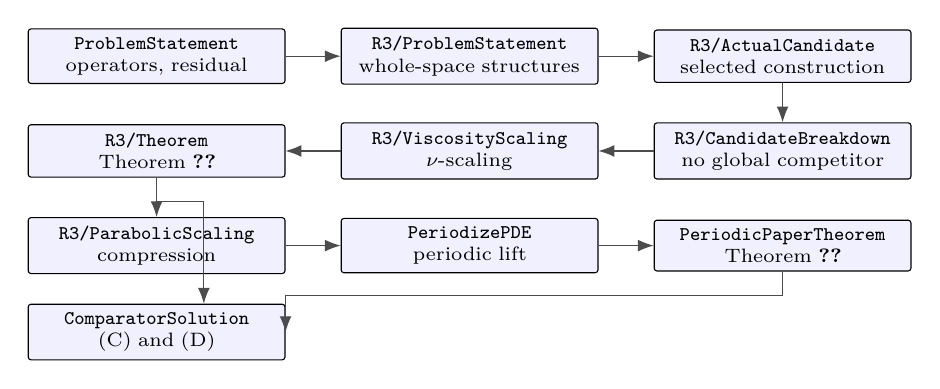
\begin{tikzpicture}[node distance=5mm and 7mm,
   box/.style={draw,rounded corners=1pt,fill=blue!6,align=center,font=\scriptsize,inner sep=3pt,text width=3.05cm},
   arr/.style={-{Latex[length=2mm]},draw=black!70}]
 \node[box] (ps) {\file{ProblemStatement}\\operators, residual};
 \node[box,right=of ps] (r3ps) {\file{R3/ProblemStatement}\\whole-space structures};
 \node[box,right=of r3ps] (act) {\file{R3/ActualCandidate}\\selected construction};
 \node[box,below=of act] (brk) {\file{R3/CandidateBreakdown}\\no global competitor};
 \node[box,left=of brk] (vis) {\file{R3/ViscosityScaling}\\$\nu$-scaling};
 \node[box,left=of vis] (thm) {\file{R3/Theorem}\\Theorem~\ref{thm:ns-r3}};
 \node[box,below=of thm] (par) {\file{R3/ParabolicScaling}\\compression};
 \node[box,right=of par] (pp) {\file{PeriodizePDE}\\periodic lift};
 \node[box,right=of pp] (pc) {\file{PeriodicPaperTheorem}\\Theorem~\ref{thm:ns-torus}};
 \node[box,below=of thm,yshift=-11mm] (cmp) {\file{ComparatorSolution}\\(C) and (D)};
 \draw[arr] (ps)--(r3ps); \draw[arr] (r3ps)--(act); \draw[arr] (act)--(brk);
 \draw[arr] (brk)--(vis); \draw[arr] (vis)--(thm);
 \draw[arr] (thm)--(par); \draw[arr] (par)--(pp); \draw[arr] (pp)--(pc);
 \draw[arr] (pc.south) -- ++(0,-3mm) -| (cmp.east);
 \draw[arr] (thm.south) -- ++(0,-3mm) -| ([xshift=6mm]cmp.north);
\end{tikzpicture}
\end{center}

The Euler chain is different in kind: the non-continuation statement
(Theorem~\ref{thm:euler-bkm}) is a corollary of the quantitative one
(Theorem~\ref{thm:euler-quant}) through the Beale--Kato--Majda criterion, and the
quantitative statement is assembled from the iteration.

\subsection{Naming and documentation}
\label{sec:naming}

Two conventions carried the development and are worth recording.

\emph{Names say what is being proved, not where it is used.}
There are modules called \file{ReservedPatches}, \file{ExponentLedger},
\file{FiveProfileMoments}, \file{MeanLocalDefectBounds}, \file{OutgoingEntranceCone},
\file{SignedRequestContinuation}. A reader who knows the source paper can find the Lean
counterpart of a numbered proposition by looking for the object it is about. This is the
opposite of a ``Chapter3\_Lemma7'' convention, and it is the right choice at this scale.

\emph{Module docstrings state the role, and often the caveat.}
\file{NavierStokes/ExponentLedger.lean} opens with ``The candidate manuscript,
Proposition 10.3, assigns real exponents to analytic estimates. This file checks the
arithmetic of those assignments, conditional on the estimates being valid. It does not
define the analytic classes, construct a correction, or prove an estimate for a PDE.''
A formalization whose docstrings say what they do \emph{not} prove is much easier to audit
than one whose docstrings only advertise.

\subsection{Dead code, removed}
\label{sec:cleanup}

Reachability analysis from the repository's entry points
(\file{NavierStokes.lean}, \file{Euler.lean}, \file{Euler/Solution.lean},
\file{ComparatorChallenges/NavierStokes.lean}, \file{ComparatorChallenges/Euler.lean},
\file{NavierStokes/TauCetiBridge.lean}) left 75 modules that no entry point reaches. 74 of
them were deleted during the migration---26{,}089 lines, 4.0\% of the tree:

\begin{center}\small
\begin{tabular}{@{}lrr@{}}
\toprule
 & files & lines \\
\midrule
before & 2{,}659 & 643{,}986 \\
removed (\lean{*NoOptions*} copies of existing modules, in a separate namespace) & 11 & 7{,}032 \\
removed (investigations and orphaned fragments of earlier constructions) & 63 & 19{,}057 \\
after & 2{,}585 & 617{,}967 \\
\bottomrule
\end{tabular}
\end{center}

The deletion is safe by construction rather than by inspection: no remaining file imports any
of the removed modules, which was checked after the removal (zero dangling imports), so no
reachable declaration changed meaning. It is also reversible with a single \lean{git revert}.
The one unreachable module that was kept is \file{NavierStokes/TauCetiBridge.lean}, which is
deliberately a leaf.

This is the only substantial reduction of code available in the repository, and it is worth
being precise about why. Removing dead code took out 4\% of the lines at zero risk. Replacing
project code by library code would take out 162 lines (the two ``free'' files of
Table~\ref{tab:infra}) plus part of nine others, and carries the risk of touching
declarations the unfinished build depends on. The remaining 99\% of the code is not
duplicated library material and cannot be reduced by substitution; it is the proof.

\section{What is verified, and how}
\label{sec:verification}

\subsection{No gaps}
\label{sec:nogaps}

A search of all 2,659 Lean files for the token \lean{sorry} returns five occurrences.
One is inside a docstring. The other four are in
\file{ComparatorChallenges/NavierStokes.lean} (lines 277 and 284) and
\file{ComparatorChallenges/Euler.lean} (lines 88 and 184), i.e.\ in the \emph{challenge
statements} that reproduce the Formal Conjectures placeholders for the Millennium problem.
Those four are not used by any proof: the challenge modules import only \Mathlib, and
nothing imports them. The two proof libraries contain no \lean{sorry}. A search for
\lean{axiom}, \lean{native\_decide}, \lean{implemented\_by}, \lean{@[extern]},
\lean{unsafe}, \lean{partial} and \lean{opaque} finds none in \file{NavierStokes/} or
\file{Euler/} either; the occurrences of the word ``axiom'' in those directories are
docstrings explaining that something is \emph{not} an axiom, for example
\file{NavierStokes/ProblemStatement.lean}: ``There is no proof, witness, or axiom
asserting this proposition in this module.''

\subsection{Axioms}
\label{sec:axioms}

The four headline declarations carry explicit \lean{\#print axioms} commands in the
repository: \file{NavierStokes/ComparatorSolution.lean} lines 31--32 for the two
Navier--Stokes alternatives, and \file{Euler/Solution.lean} lines 73 and 75 for the two
Euler statements. The reported dependency sets are
\[
  \{\lean{propext},\ \lean{Classical.choice},\ \lean{Quot.sound}\},
\]
the standard classical base of \Mathlib{} analysis. Section~\ref{sec:migration-results}
reports the same commands re-run after the migration.

We re-ran those commands at the pinned toolchain after the migration, and can now report
the compiler's own answer rather than the repository's claim:

\begin{lstlisting}[language=ML]
'NavierStokesR3.breakdownStatement' depends on axioms: [propext, Classical.choice, Quot.sound]
'NavierStokes.PeriodicPaper.breakdownStatement' depends on axioms: [propext, Classical.choice, Quot.sound]
'NavierStokes.Comparator.navier_stokes_breakdown_R3' depends on axioms: [propext, Classical.choice, Quot.sound]
'NavierStokes.Comparator.navier_stokes_breakdown_periodic' depends on axioms: [propext, Classical.choice, Quot.sound]
\end{lstlisting}

This matters more than it might appear. A formalization of this size has many places
where a proof could in principle be closed by a stronger assumption---an inverse function
theorem asserted as an axiom, a well-posedness theorem assumed for the class at hand. The
axiom audit is what rules that out: an unproved input would show up as an extra axiom in
the dependency set of the headline theorem, and there is none.

\subsection{Statement fidelity}
\label{sec:fidelity}

Typechecking a theorem says nothing about whether it states the intended mathematics. We
checked the statements in three ways.

\emph{Definitions copied, not paraphrased.} The Euler definitions
(\file{Euler/SolutionDefinitions.lean}) and both challenge modules are adapted from the
Formal Conjectures formalization of the Millennium problem statement, with a comment
recording the upstream commit. The task was therefore to prove \emph{that} statement, not
a convenient variant.

\emph{Every hypothesis is explicit.} The Navier--Stokes statement's force class, for
example, is \lean{CompactPositiveTimeSupport f}, defined as
\lean{HasCompactSupport f ∧ tsupport f ⊆ Ioi 0 ×ˢ univ}: smooth, compactly supported in
spacetime, supported at strictly positive times. The energy condition is
\lean{UniformFiniteEnergy (Ico 0 1) u}, which asks for a single $E\ge0$ with
\lean{SquareIntegrableAtTime u t} and \lean{kineticEnergy u t ≤ E} for every $t\in[0,1)$.
Neither condition can be satisfied vacuously, and neither hides an assumption about the
\emph{competitor}, which is quantified with no support, growth or energy-inequality
hypothesis beyond the bound.

\emph{No statement is vacuous.} The two constructions are explicit: the repository builds
the fields and then proves the properties, so the existential statements have witnesses
that can be inspected. Theorems that are only \emph{conditional} are named as such; for
example \file{NavierStokes/ProblemStatement.lean} contains the proposition
\lean{candidateStatement} together with a docstring saying that nothing in the module
proves it, and the proof that it holds is in \file{NavierStokes/R3/Theorem.lean} under the
same name. This is a good convention: a reader who searches for a statement finds, at the
statement, a pointer to where it is discharged.

\subsection{Independent checking}
\label{sec:comparator}

The repository ships a Comparator configuration (\file{ComparatorChallenges/}), which
exports the four headline theorems to Lean's kernel-independent proof format and replays
them through a separate checker after translation. This is a defence against a bug in
Lean's own kernel or in the elaborator, and it is the strongest available form of
independent verification for a Lean development. The migration described in
Section~\ref{sec:libraries} forced a choice here: Comparator is released per toolchain and
its releases stop at \Lean{} \texttt{v4.35.0}, one version below the toolchain that
\TauCeti{} requires. We kept the migration and the challenge definitions and dropped the
Comparator \emph{library} dependency; the challenge files remain in the repository and can
be re-checked with a Comparator installation matching whichever toolchain is in use.

\section{The library migration}
\label{sec:libraries}

The repository was written against Lean \texttt{v4.34.0-rc2} and the \Mathlib{} commit that
toolchain fixes. This section documents its migration to the current library generation and
to \TauCeti{}, and reports what the move cost.

\subsection{The target pin}
\label{sec:pin}

Two upstream constraints determine the possible targets. \TauCeti{} pins a toolchain and a
\Mathlib{} commit, and Lake refuses to build a package whose dependencies disagree about the
toolchain. At the time of writing \TauCeti{} is on Lean \texttt{v4.36.0-rc1} with \Mathlib{}
at \texttt{2cabef97}; the newest \Mathlib{} release is \texttt{v4.36.0-rc2}, whose toolchain
no \TauCeti{} release uses. We therefore chose the pin that is simultaneously the newest
\TauCeti{} and the newest \Mathlib{} that \TauCeti{} supports:
\begin{center}
\begin{tabular}{@{}lll@{}}
\toprule
component & old pin & new pin \\
\midrule
Lean & \texttt{v4.34.0-rc2} & \texttt{v4.36.0-rc1} \\
\Mathlib{} & \texttt{v4.34.0-rc2} & \texttt{2cabef97b63d} \\
\TauCeti{} & --- & \texttt{b8cbc774e9a4} \\
Comparator & \texttt{v4.34.0-rc2} & dropped (see below) \\
\bottomrule
\end{tabular}
\end{center}
The \lean{rev} fields are full commit hashes rather than branch names, so that
\lean{lake update} is deterministic; \lean{lakefile.toml} records the reason for each pin in
a comment.

\paragraph{Comparator.} Comparator is released per toolchain, and its releases stop at
\Lean{} \texttt{v4.35.0}, one toolchain below the one \TauCeti{} requires. Since Comparator is
needed only for the independent re-checking of the four headline theorems and not for their
proofs, we removed it from the dependency set. The two challenge modules and their JSON
configurations remain in the repository unchanged---they import only \Mathlib{}---so
independent checking is still possible with a Comparator installation matching whichever
toolchain is in use. This is the one place where the migration cost functionality rather
than just time, and it is recorded in \file{MIGRATION.md}.

\subsection{Practical obstacles}
\label{sec:obstacles}

The migration is not a version bump; it is a small research project in code archaeology. The
obstacles we met, in decreasing order of the number of sites they affected, were the
following.

\paragraph{\lean{MemLp} became a definition.} In the pinned \Mathlib{}, \lean{MemLp f p μ}
is \emph{defined} to be \lean{eLpNorm f p μ < ∞} rather than a structure with a
measurability field and a finiteness field. Consequently:
\begin{itemize}
\item field projections \lean{hf.1}, \lean{hf.2} must become the lemmas
      \lean{hf.aestronglyMeasurable} and \lean{hf.eLpNorm\_lt\_top};
\item anonymous-constructor terms \lean{⟨hmeas, hbound⟩} of type \lean{MemLp f p μ} must
      become the finiteness proof alone;
\item any \lean{obtain ⟨hmeas, hfin⟩ := hf} must be rewritten.
\end{itemize}

\paragraph{Measurability hypotheses moved in and out of the \texorpdfstring{$L^p$}{Lp} API.}
This is the subtle one. \lean{eLpNorm} used to be $0$ for non-a.e.-strongly-measurable
functions, which made monotonicity lemmas unconditional; it is now $\infty$ in that case,
so \lean{eLpNorm\_mono\_ae} gained an explicit measurability hypothesis and
\lean{eLpNorm\_one\_eq\_lintegral\_enorm} became a lemma \emph{with} a hypothesis. In the
other direction, \lean{eLpNorm\_add\_le} \emph{lost} its two measurability arguments and now
takes only the exponent hypothesis \lean{1 ≤ p}. A proof that says
\lean{eLpNorm\_add\_le hf.aestronglyMeasurable hg.aestronglyMeasurable hp1} must become
\lean{eLpNorm\_add\_le hp1}, while a proof that says \lean{eLpNorm\_mono\_ae h} must become
\lean{eLpNorm\_mono\_ae hf h}---possibly with a case split, because the measurability of the
dominated function is genuinely no longer automatic. One project lemma
(\lean{lpNorm\_mono\_of\_norm\_le\_ae}) acquired a proof by cases on measurability for exactly
this reason, and a hypothesis of the corresponding library statement was thereby
strengthened: a semantic change forced by the library, not a syntactic one.

\paragraph{One change is not a repair but a gap.} The most interesting failure
found by the migration is in \file{Euler/EulerProof.lean}. Five proofs there apply
\lean{eLpNorm\_le\_mul\_eLpNorm\_of\_ae\_le\_mul} to an \emph{iterated field derivative}, with no
measurability hypothesis in hand, because under the old convention \lean{eLpNorm} was $0$ on
functions that are not a.e.\ strongly measurable and the inequality was therefore free. Under
the pinned library \lean{eLpNorm} is $\infty$ there, so the lemma needs measurability of that
derivative, and the development has no lemma producing it: the smoothness it proves is
smoothness of the \emph{lifted local field}, not measurability of the derivative-valued map on
the domain. The proofs are not syntactically broken; they are correct only under an
assumption the library no longer makes, and closing them means proving a measurability lemma
that the development never needed. This is the clearest instance in the whole migration of a
library change that alters what has to be proved rather than how it is written, and it is why
the residual error count in \file{EulerProof} should not be read as a measure of remaining
effort.

\paragraph{Explicit exponent hypotheses became a structure.}
\lean{eLpNorm'\_le\_eLpNorm'\_mul\_eLpNorm'} (the interpolation inequality for
\lean{eLpNorm'}) previously took the three exponent facts as separate arguments; it now takes
a single \lean{Real.HolderTriple p q r}, and its two measurability arguments moved from the
front to the middle of the argument list. Interpolation sites must be rewritten to build the
structure:
\begin{lstlisting}
have hpqr : Real.HolderTriple (p.toReal / a) (q.toReal / b) r.toReal :=
  { inv_add_inv_eq_inv := by simpa only [one_div] using hab.symm
    left_pos := div_pos hp hpt ha
    right_pos := div_pos hq hqt hb }
simpa using eLpNorm'_le_eLpNorm'_mul_eLpNorm'
  (fun x y : ℝ => x * y) 1
  (hf.norm.aemeasurable.pow_const a).aestronglyMeasurable
  (hg.norm.aemeasurable.pow_const b).aestronglyMeasurable
  (Filter.Eventually.of_forall fun x => by simp [nnnorm_mul])
  hpqr
\end{lstlisting}

\paragraph{Hidden arguments became explicit and vice versa.}
\lean{contDiff\_apply} now takes the differentiability order implicitly, so every application
in a fixed-order context must say \lean{(n := ∞)}; \lean{norm\_iteratedFDeriv\_fderiv}
changed from ``$\|D^n(\mathrm{d}f)\| = \|D^{n+1}f\|$'' to a form in which the dependent
function is implicit, so a two-argument application must be replaced by an explicitly typed
\lean{have}; \lean{Finset.prod\_le\_prod} now demands a \lean{MulLeftMono} instance that
$\mathbb{R}$ does not have, so a monotonicity proof for a product of factors of the form $b+k$
must be restated so that positivity of the factors is available.

\paragraph{The module system.}
\Lean{} \texttt{v4.36} introduces the module system: a file opened with \lean{module} may
\lean{public import} and hides its non-public declarations. \Mathlib{} and \TauCeti{} have
adopted it, and Lean emits a warning for every import of a module file from a file that has
not declared itself a module:
\begin{lstlisting}
warning: NavierStokes/R3/ComparisonGronwall.lean: imports
  `Mathlib.Analysis.Calculus.Deriv.MeanValue` from package `mathlib`, which is designed for
  use with the module system; consider adding `module` to the start of this file
\end{lstlisting}
The warnings are harmless, but they are also loud: at this scale they run to several per
file. Adding a \lean{module} header to every file makes them disappear and puts the
repository on the same footing as its dependencies; a \lean{module} file cannot import a
non-\lean{module} file, so the change is all-or-nothing.

\subsection{\TauCeti{}: what it supplies}
\label{sec:tauceti}

\TauCeti{} is a downstream analysis library organised along the same lines as \Mathlib{}
itself: 2{,}793 files under \file{TauCeti/Analysis/}, of which the areas relevant here are
Sobolev theory (142 files: weak derivatives, Bessel potentials, embeddings, mollification,
Poincaré, Rellich--Kondrachov, trace theory on Lipschitz domains), PDE (161 files:
fundamental solutions, Green functions, the heat kernel with its semigroup and Duhamel
potential, Caccioppoli and Harnack estimates), distributions (56 files: Schwartz space,
Littlewood--Paley, tempered distributions, Fourier multipliers), Fourier theory (42 files)
and parametric integration. It is built on \Mathlib{} and uses the module system throughout.

For this repository the interesting entry points are these.

\begin{center}\small
\begin{longtable}{@{}p{0.36\textwidth}p{0.58\textwidth}@{}}
\toprule
\TauCeti{} module & relevance \\
\midrule
\file{Analysis/Calculus/ParametricIntegral} & $C^n$ regularity of compact-parameter
integrals, iterated derivatives under an interval integral with individually bounded
derivatives; replaces the project's \file{SmoothParameterIntegral} and
\file{CompactParameterIntegral} \\
\file{Analysis/Sobolev/Mollification} & the mollification identity
$D_v(u\star\rho) = u'\star\rho$ for weak derivatives, followed by density \\
\file{Analysis/Sobolev/Embedding}, \file{Morrey}, \file{LipschitzDomain/*} & Sobolev
embeddings, trace and extension theorems on Lipschitz domains \\
\file{Analysis/PDE/HeatKernel/*} & heat kernel, semigroup, smoothing, Duhamel potential
--- the analytic core of the exterior swirl field \\
\file{Analysis/Distribution/SchwartzSpace/LittlewoodPaley} & frequency localisation at the
level the dyadic charts use informally \\
\file{Analysis/Fourier/MihlinHormander} & Fourier-multiplier bounds for the pressure
recovery \\
\bottomrule
\end{longtable}
\end{center}

\subsection{What can actually be replaced}
\label{sec:replace}

It is easy to overstate this. The project's analysis is not organised the way a textbook
library is organised: its Sobolev spaces are word lattices over a cylinder designed to be
complete \emph{as defined}, its cutoffs are built with explicit all-order bounds tied to
reserved logarithmic patches, and its heat kernel is tied to a specific radial similarity
ansatz. Replacing such objects wholesale would be a redesign of the development, not a
migration. What is genuinely replaceable divides into three classes.

\emph{Replaceable now, because the statement matches.} Compact-parameter integration is the
clearest case: \TauCeti{} proves exactly the regularity statement the project needs and
proves it for a general compact parameter space with a weight, which is strictly more general
than the project's version. Smooth functions with prescribed support are another: the project
constructs its own bump and cutoffs from $\exp(-1/x)$, while both \Mathlib{} and \TauCeti{}
already provide them.

\emph{Replaceable after a statement change.} The project defines Sobolev spaces of all
orders on a cylinder as a lattice of words to obtain completeness without a completion; a
library Sobolev space is a predicate on distributions. Moving to the library notion would
change the meaning of the objects the estimates are about, so this is a refactoring of the
Euler development rather than a substitution, and it should be done (if at all) only with the
estimates in view.

\emph{Not replaceable today.} The weighted band-indexed coefficient classes $W_\alpha$,
$M_\alpha$, $S_\alpha$ of the Navier--Stokes construction, the pulse envelopes and their
logarithmic edge weights, and the exponent ledger \eqref{eq:sigma} are bespoke objects of
this proof. A library would not want them.

\subsection{Outcome of the migration}
\label{sec:migration-results}

The dependency move itself is complete: the repository resolves, \Mathlib{}'s oleans are
fetched from the cache (9{,}057 files, about 4.8\,GB of build artifacts, under a minute on
a warm connection), and \TauCeti{}'s own modules build from its published cache (5{,}521
jobs, nine seconds). What remains is the repair of the project's own 644k lines against the
new API.

We worked through the failures reported by the compiler file by file. The sites we
repaired, and the shape of each repair, are the following.

\begin{center}\small
\begin{longtable}{@{}p{0.36\textwidth}p{0.58\textwidth}@{}}
\toprule
file & repair \\
\midrule
\file{R3/LpNormTools} & \lean{MemLp} projections; \lean{eLpNorm\_add\_le} lost its
  measurability arguments; \lean{eLpNorm\_one\_eq\_lintegral\_enorm} gained one; one lemma
  reproved by cases on measurability \\
\file{R3/PairedKernelBound} & the same, plus \lean{eLpNorm\_smul\_le\_mul\_eLpNorm}
  reordered (the scalar field comes first) and \lean{eLpNorm\_norm} needing its hypothesis \\
\file{R3/WeightedInterpolation} & \lean{Real.HolderTriple} construction; a measurability
  hypothesis added to the interpolation lemma and threaded to its call site;
  \lean{eLpNorm\_eq\_eLpNorm'} now needs its function named explicitly \\
\file{R3/PressureFunctionals}, \file{R3/H3Products} & \lean{MemLp} projections replaced by
  \lean{hf.aestronglyMeasurable} \\
\file{R3/ComparisonCutoffs} & \lean{norm\_iteratedFDeriv\_fderiv} restated with an explicit
  type; \lean{Finset.prod\_le\_prod} replaced by \lean{gcongr} \\
\file{AppendixHeatResults} & the same \lean{gcongr} replacement for a product of linear factors \\
\file{R3/ComparisonFiniteEnergy} & \lean{MemLp} projections (\lean{hf.1} to
  \lean{hf.aestronglyMeasurable}), including on a difference \lean{hf.sub\ hg} \\
\file{EdgeWeightJets}, \file{WeightedRadialPrimitive} & \lean{Finset.prod\_le\_one} needs
  \lean{MulLeftMono}, which $\mathbb{R}$ lacks; replaced by writing the product of equal
  factors as a power and using \lean{pow\_le\_one\textsubscript{0}} \\
\file{SmoothCovariance}, \file{SquaredPartition} & \lean{contDiff\_apply} and
  \lean{contDiff\_apply\_apply} now take the order implicitly and the family explicitly:
  \lean{contDiff\_apply\ \mathbb{R}\ (fun\ \_\ =>\ \mathbb{R})\ i} \\
\file{TauCetiBridge} (new) & imports \TauCeti{} and restates its parametric-integration
  theorems at project names; requires \lean{[CompleteSpace\ F]} on the codomain \\
\bottomrule
\end{longtable}
\end{center}

\paragraph{Status.} \textbf{The \file{NavierStokes} library builds.} Under the pinned
toolchain, \lean{lake build NavierStokes} completes with 19{,}645 jobs and exit code $0$ and no
diagnostics of any kind: all 816 modules elaborate. The two challenge modules of
\file{ComparatorChallenges} build as well (18{,}136 jobs), so of the repository's three
targets only \file{Euler} fails. Fifteen rounds of repair took it from 228
modules to the whole library, and no theorem statement was modified --- every change is a
proof, an explicit implicit argument, or, in exactly one place, a measurability hypothesis
added to a private helper lemma (\lean{lpNorm\_ofReal}) because the library lemma it calls now
demands one.

Two things made the difference, and both are worth recording for anyone else doing this.
First, \emph{read the goals, do not guess them}: inserting \lean{trace\_state} before each
failing line showed that the set a \lean{mono} expects is usually an intermediate one
manufactured by an enclosing \lean{apply}, not the theorem's own set. On that evidence the
eleven failures in \file{NominalProfile} fell in one pass, after two earlier attempts had
guessed wrong and made the file worse. Second, \emph{the two \lean{mono} lemmas do not name
their sets alike}:
\[
  \lean{IntegrableOn.mono\_set}\ (h : \lean{IntegrableOn}\ f\ t\ \mu)\ (hst : s \subseteq t)
  \quad\text{and}\quad
  \lean{ContDiffOn.mono}\ (h : \lean{ContDiffOn}\ f\ s)\ \{t\}\ (hst : t \subseteq s),
\]
so the target is \lean{s} in the first and \lean{t} in the second. Seven of the eleven sites
needed \lean{(s\ :=\ ...)} and four \lean{(t\ :=\ ...)}; applying one convention to all of them
does nothing and looks as though the argument had been ignored.

The \file{Euler} library is a different story and we do not dress it up. Its 1{,}839 modules
stand at 42 elaborated; \file{Euler/EulerProof} rejects 28 sites, five of which need a
measurability lemma the development never had (see below), three are \lean{case hf}
hypotheses, two are \lean{ContinuousAdd} instances that no longer resolve, and eighteen are
one-offs spread over 20{,}755 lines.


\subsection{How much of this duplicates the libraries?}
\label{sec:dup}

It is natural to suspect that a development of this size, written quickly against a large
library, consists largely of re-proved library facts. We tested the suspicion, and it is
false, but the measurement is worth reporting because the way in which it is false is the
interesting part.

\paragraph{Name overlap.} Extracting every \lean{theorem}, \lean{lemma}, \lean{def},
\lean{abbrev} and \lean{instance} name from the three trees gives 43{,}101 declarations
here, 170{,}982 in \Mathlib{} (at the pinned commit) and 237{,}302 in \TauCeti{}. The count
for this repository was taken before the unused-lemma removal of
Section~\ref{sec:unused}; that removal deletes 6{,}328 declaration names, and repeating the
two exact-match rows on the pruned tree gives 422 (1.1\%) and 513 (1.4\%)---the shares move
by a tenth of a percentage point, which is the size of the effect that a 12\% reduction in
code has on this measurement.

\begin{center}\small
\begin{tabular}{@{}lrr@{}}
\toprule
comparison & declarations & share of the development \\
\midrule
exact name also in \Mathlib{} & 438 & 1.0\% \\
exact name also in \TauCeti{} & 531 & 1.2\% \\
base name also in \Mathlib{} & 829 & 1.9\% \\
base name also in \TauCeti{} & 899 & 2.1\% \\
base name in either & 1{,}159 & 2.7\% \\
\bottomrule
\end{tabular}
\end{center}

Name matching is a weak proxy and it cuts both ways: the project names things
descriptively (\lean{jetPolynomial}, \lean{majorant\_mul}, \lean{rising\_mono}), so semantic
duplication is under-counted.

\paragraph{Where the duplication actually is.} The infrastructure layer is the answer. Of
the 2{,}588 files, eighteen---3{,}855 lines, 0.7\% of the lines---rebuild
standard analysis: smooth cutoffs with all-order bounds, the exponential edge
$\exp(-c/x^2)$, zero extension across it, finite-order jet bookkeeping, the Banach space
$C^k([-1,1];E)$, differentiation under the integral sign (twice, in incompatible forms),
Schwartz density, $L^2$ mollification, word-lattice Sobolev spaces, and the derivative gain
of the heat kernel. That is where \TauCeti{} overlaps, and that is the entire target set for
a library migration. The remaining 99.4\% of the code has no counterpart in any library,
because it is the proof: the profiles, the dyadic charts, the reserved patches, the pulse
covariances, the correction stages, the packet frames.

\paragraph{Duplication of the development with itself.} A different and more serious
question is internal duplication, and here the answer is less comfortable: 74 modules are
unreachable from any entry point (Section~\ref{sec:cleanup}), eleven of them literal copies
of other modules placed in a separate namespace so that a heavy proof could be re-elaborated
under different heartbeat limits, and the same argument is proved twice in
\file{SmoothParameterIntegral} and \file{CompactParameterIntegral} because the two files
were written independently. Internal duplication, not library duplication, is the real
technical debt here.

\paragraph{Measuring it properly.} The right instrument is a type-level comparison, not a
name-level one: \Mathlib{} ships \file{Mathlib/Tactic/DuplicateDecls.lean} (Gerbscheid),
which normalises every theorem type by erasing universes and sorting binders, then hashes
the result, so that two theorems count as duplicates when their statements agree up to
binder order, binder information and universe levels. It cannot be used as shipped---its
declarations are not \lean{public} in the module system, so an importing file cannot call
them---and we vendored the forty lines of its core into a probe.

We validated the probe before trusting it, and the validation is the reason the numbers
below are worth reporting. Two controls were placed in a separate module: \lean{plantedA}
and \lean{plantedB}, the theorems $n=n$ and $m=m$, which duplicate each other; and
\lean{plantedAddComm}, stating $a+b=b+a$, which duplicates \Mathlib's \lean{Nat.add\_comm}.
The probe found exactly two groups involving a project declaration: \lean{[plantedA,
plantedB]} and \lean{[Nat.add\_comm, plantedAddComm]}. It sees what it claims to see.

Running it over 22 of the repository's modules---the infrastructure layer and the first
\file{NavierStokes} files, i.e.\ deliberately sampling where duplication with a library is
most likely---gives:

\begin{center}\small
\begin{tabular}{@{}lr@{}}
\toprule
theorem-duplicate groups in the environment & 1{,}533 \\
project theorems passing the filters & 802 \\
groups involving a project theorem & 2 (both planted controls) \\
groups involving a project theorem, controls removed & \textbf{0} \\
\bottomrule
\end{tabular}
\end{center}

The two counts above the line are lower than in the first measurement of this tree (2{,}401
groups, 944 theorems) because the unused-lemma removal of Section~\ref{sec:unused} took
142 theorems out of the sample as well (6{,}330 out of the tree); the number that matters,
the last row, is unchanged at zero.

So not a single theorem in the sample restates a library theorem, even up to binder
reordering. This does not contradict the infrastructure finding above: the duplication that
exists is duplication of \emph{concepts}, not of statements. \lean{SmoothCutoffs.one\_le\_growth}
is not any \Mathlib{} lemma; it is a bespoke weighted bound whose role a library would
express differently. The cost of that is real, but it is not measured by counting shared
theorems, and the migration effort should be directed by the concept-level audit of
Section~\ref{sec:replace}, not by a duplicate-declaration report.

\paragraph{The probe as a regression check.} Both the probe and its controls are kept in
the repository, in \file{scripts/DuplicateProbe.lean} and
\file{scripts/PlantedControls.lean}; they are outside every library target, so they cost
nothing at build time. Rerunning the probe after a refactoring is cheap and it is the only
mechanical defence against the drift that the \TauCeti{} roadmap warns about: a standard
notion said in the project's own dialect grows a redundant theory of lemmas the library
already proves. The probe measures the narrow, syntactic form of that drift. The conceptual
form---reimplementing a notion with a different statement---is what the table in
Section~\ref{sec:replace} catalogues, and no automated tool replaces reading the files.

\subsection{The eighteen infrastructure files, one by one}
\label{sec:infra-table}

Table~\ref{tab:infra} is the concrete form of the claim made above. It lists every file of
the infrastructure layer with its size, what it builds, the closest library artefact, and a
verdict. The verdicts are: \emph{free} if the project's statement is the library's statement
and a one-line restatement suffices; \emph{partial} if the library covers part of the file or
covers it under hypotheses that have to be discharged; \emph{keep} if the object is
project-specific and a library would not want it; and \emph{notion} if the library has a
theory of the same name but a different object, so that replacement is a redesign rather
than a substitution.

\begin{center}\scriptsize
\begin{longtable}{@{}p{0.235\textwidth}rrp{0.205\textwidth}p{0.215\textwidth}p{0.09\textwidth}@{}}
\caption{The eighteen infrastructure files, what they build, the closest library artefact and
a verdict.}\label{tab:infra}\\
\toprule
file & lines & decls & what it builds & library counterpart & verdict \\
\midrule
\endfirsthead
\toprule
file & lines & decls & what it builds & library counterpart & verdict \\
\midrule
\endhead
\file{NavierStokes/}\newline\file{SmoothCutoffs} & 309 & 35 & smooth cutoffs on balls and
  strips, all-order derivative bounds, time switch & \Mathlib{} \lean{ContDiffBump},
  \lean{expNegInvGlue}; \TauCeti{} \file{BumpFunction/Cutoff} & free \\
\file{NavierStokes/}\newline\file{FlatCutoff} & 204 & 26 & the edge $\exp(-c/x^2)$ and its
  inverse-power family $x^{-\ell}\exp(-c/x^2)$ & \Mathlib{} \lean{expNegInvGlue}
  (\emph{without} the $c$-family) & partial \\
\file{NavierStokes/}\newline\file{FlatZeroExtension} & 243 & 21 & zero extension of a jet
  across such an edge & none & keep \\
\file{NavierStokes/}\newline\file{JetBounds} & 311 & 27 & finite-order bounds on
  \lean{iteratedFDeriv}, Leibniz profile & \Mathlib{} \lean{norm\_iteratedFDerivWithin\_mul\_le};
  \TauCeti{} \file{IteratedFDeriv/Basic} & partial \\
\file{NavierStokes/}\newline\file{WeightedClasses} & 517 & 37 & the weighted band-indexed
  coefficient classes $W_\alpha,M_\alpha,S_\alpha$ & none & keep \\
\file{NavierStokes/}\newline\file{ClosedIntervalCk} & 337 & 34 & the Banach space
  $C^k([-1,1];E)$ as a closed submodule of jet data & none (\TauCeti{}
  \file{IteratedDerivWithin} is pointwise, not a space) & keep \\
\file{NavierStokes/}\newline\file{ClosedIntervalJetAlgebra} & 293 & 31 & polynomial
  expressions in jets and their bounds & \Mathlib{} \lean{MvPolynomial} plus a bespoke
  interval-arithmetic interpreter & partial \\
\file{NavierStokes/}\newline\file{SmoothParameterIntegral} & 315 & 20 & all-orders
  differentiation under an integral over an arbitrary measure space & \TauCeti{}
  \file{Calculus/ParametricIntegral} covers the compact-parameter case & partial \\
\file{NavierStokes/}\newline\file{SchwartzCompactApproximation} & 58 & 4 & quantitative
  density of compactly supported smooth functions in $\mathcal S$, and the consequence that
  compact tests determine a tempered distribution & \TauCeti{} \lean{SchwartzMap.dense\_hasCompactSupport}
  & \textbf{done} \\
\file{Euler/}\newline\file{OrdinaryMollifier} & 164 & 26 & $L^2$-valued mollification along
  an isometric action, with rate & \TauCeti{} \file{Sobolev/Mollification} proves the
  weak-derivative identity instead & notion \\
\file{Euler/}\newline\file{CylinderSobolevSpace} & 145 & 25 & Sobolev spaces of all orders on
  a cylinder as a lattice of derivative words, complete by construction & \TauCeti{}
  \file{Sobolev/*} and \Mathlib{} \lean{BesselPotentialSpace} are Fourier-based and
  predicate-level & notion \\
\file{Euler/}\newline\file{SobolevWordLevel} & 54 & 5 & the level structure of that lattice &
  none & keep \\
\file{Euler/}\newline\file{SobolevSmoothApproximation} & 109 & 11 & smooth approximation in
  the word-lattice topology & \TauCeti{} \file{Sobolev/Mollification/Interior} (different
  carrier) & notion \\
\file{Euler/}\newline\file{SobolevHeatKernel} & 156 & 11 & heat gain of $k$ derivatives with
  an explicit parabolic majorant & \TauCeti{} \file{PDE/HeatKernel/Smoothing} (different
  carrier) & partial \\
\file{Euler/}\newline\file{CompactParameterIntegral} & 74 & 5 & $C^\infty$ parametric
  integral over a compact interval, from \emph{local} boundedness of the derivatives &
  \TauCeti{} \file{Calculus/ParametricIntegral} asks for bounds \emph{uniform in $x$}, which
  joint smoothness does not give; only the \lean{ContDiffOn} variant applies & partial \\
\file{Euler/}\newline\file{LpBochnerRealization} & 88 & 6 & $L^2(\mu;L^2(\nu))\cong
  L^2(\mu\otimes\nu)$ with equality of norms & \Mathlib{} \lean{MeasureTheory.Lp},
  \lean{integrable\_prod\_iff}; the identification is a short consequence & free \\
\file{Euler/}\newline\file{FiniteGradeAlgebra} & 109 & 10 & a truncated graded algebra with
  evaluation and a convolution inverse & \Mathlib{} \lean{Polynomial} evaluation and
  \lean{Finset.sum\_range} algebra & partial \\
\file{NavierStokes/}\newline\file{AppendixHeatResults} & 177 & 12 & rising factorials,
  $\Gamma(b+n)$ recursion, endpoint jets of the radial heat profile & \Mathlib{}
  \lean{ascPochhammer}, \lean{Real.Gamma\_add\_one}; \lean{rising} is now
  \lean{(ascPochhammer\ \mathbb{R}\ n).eval\ b} & \textbf{done} \\
\midrule
total & 3{,}674 & 387 & & & \\
\bottomrule
\end{longtable}
\end{center}
\noindent The verdict \lean{free} means a one-line restatement suffices; \lean{partial}
means the library covers part of the file; \lean{notion} means the library has a different
object of the same name; \lean{keep} means no library would want it.

\paragraph{What the table says.} Five substitutions have since been made, each verified by a green build.
\file{AppendixHeatResults} is done: its rising factorial \emph{is} Mathlib's
\lean{ascPochhammer} evaluated, with \lean{rising\_succ} and \lean{rising\_pos} now one-line
applications and only the monotonicity lemmas still by induction. In \file{R3/PairedKernelBound}
a duplicate of \lean{lpNorm\_one\_eq\_integral\_norm} was deleted, the file using the copy in
\file{R3/LpNormTools}. And in \file{R3/PressureFlux} the identity
$\|\mathrm{d}f(\lambda y.\,y{:}\mathbb{C})\| = \|\mathrm{d}f\|$ had been proved by an
antisymmetry argument over the operator norm in fifteen lines; it is now six, because
\Mathlib{} has \lean{LinearIsometry.norm\_toContinuousLinearMap\_comp} and
\lean{Complex.ofRealCLM} is \lean{Complex.ofRealLI.toContinuousLinearMap} by \lean{rfl}. The
net line change of those three is $+3$: what was removed is a bespoke proof, not a
statement.

The fifth is the one with volume. \file{R3/SchwartzCompactApproximation} reconstructed
density of compactly supported smooth functions in Schwartz space from a cutoff family and a
seminorm estimate---the whole file was 235 lines and 20 declarations---and nothing in the
library used the construction. \TauCeti{} proves the statement for the same object
(\lean{SchwartzMap.dense\_hasCompactSupport}, in \file{SchwartzSpace/Cutoff}), so the file
is now the import plus the two closed-set consequences of density: 235 $\to$ 58 lines,
20 $\to$ 4 declarations. Two further project theorems, \lean{image\_exp\_Iic} and
\lean{image\_exp\_Ioi}/\lean{Ioc}, were Mathlib's \lean{Real.image\_exp\_*} verbatim and are
gone, with their eleven uses repointed.

Finding these was mechanical rather than by reading. The duplicate probe of
Section~\ref{sec:dup} was run over the whole \file{NavierStokes} library instead of the
22-module sample, and it reports \emph{seven} theorem-duplicate groups involving a library
theorem: the two deliberate \TauCeti{} bridge aliases, one project--project pair, and the
four project theorems replaced above. That is the ceiling of statement-level substitution in
this library, and it is small because the library genuinely does not restate \Mathlib{}. The
Schwartz file is the one case where the duplication was of a \emph{construction} rather than
of a statement, and the probe cannot see those; it took reading the table in this section to
find it. That leaves two done, one free, eight partial, three notion-level and four to keep. (The parametric-integral file was recorded as
free in an earlier draft of this table; checking its hypotheses against \TauCeti's showed
that the library theorem needs bounds uniform in the differentiation variable, which the
project's joint-smoothness hypothesis does not supply, so it moved to \emph{partial}.) Nothing in the layer is large: the whole of it is
3{,}674 lines, which is 0.7\% of the development. The conclusion is that a library migration
of this repository is worth doing for the two free files and the eight partial ones, and is \emph{not} worth doing for the
word-lattice Sobolev spaces: those exist because the classical object was not available in
the library at the time, and replacing them now would change the meaning of the estimates
that the Euler development is made of. The honest intermediate step is the bridge lemma
\lean{SobolevSpace\ q\ →\ MemSobolev\ q\ 2}, which would connect the project's carrier to
\Mathlib's predicate and let the two theories be used side by side; it is not proved here.

\paragraph{Is any of this a special case of a general library lemma?} The duplicate probe
answers the question only for theorems whose \emph{statements} coincide. A project lemma can
also be a special case of a strictly more general library lemma, and that would be worth
replacing. To test it we asked the library directly: for each theorem, replace its proof by
\lean{exact?} \emph{in its own context} (no re-printing of types, so nothing is lost in
translation) and see whether a library term closes the goal.

The sample is the population where such a replacement is plausible: the \textbf{509}
\file{NavierStokes} theorems whose statement mentions \emph{no} project-defined constant, of
which the \textbf{173} in the 28 largest such files were run. The instrument was validated
first, on \lean{example : 0 < 2 * Real.pi := by exact?} and
\lean{example (x : ℝ) : x + 0 = x := by exact?}, which must --- and do --- report
\lean{Real.two\_pi\_pos} and \lean{AddMonoid.add\_zero}. (The first run of the harness looked
for the wrong line of \lean{exact?}'s two-line output and reported 0 of 173; the control is
what caught it.)

\textbf{9 of 173} are closed by a suggestion, and of those nine only \textbf{four} name a
library declaration:

\begin{center}\small
\begin{tabular}{@{}ll@{}}
\toprule
project theorem & library lemma that proves it \\
\midrule
\lean{real\_smul\_as\_complex\_mul} & \lean{Complex.real\_smul} \\
\lean{ae\_radial\_ne\_zero} & \lean{Measure.ae\_ne volume 0} \\
\lean{deriv\_smooth} & \lean{ContDiff.deriv'} \\
\lean{two\_le\_infty} & \lean{Std.LawfulOrderOrd.isGE\_compare} \\
\bottomrule
\end{tabular}
\end{center}

The other five suggestions are \emph{project} lemmas, which is the healthy case: the
development already factors them. All four replacements were applied; each saved one or two
lines, because each theorem was already a one-liner. The remaining 164 theorems are not
special cases of anything in the library: they are quantitative estimates about specific real
numbers, and \Mathlib{} has no general lemma to offer.

So the library overlap of this development is empty at the statement level (no theorem
duplicates a library theorem, checked against the whole of \Mathlib{}), and near-empty at the
level of generality (four one-line special cases out of 173 sampled). Whatever else accounts
for 341{,}000 lines, it is not library material.

\section{Assessment}
\label{sec:assessment}

\subsection{What the formalization shows}

The repository proves, with no axioms beyond the classical base, that the two mechanisms in
the source papers actually produce what they claim: a forced Navier--Stokes flow that stays
in bounded energy while its velocity blows up, and an unforced Euler flow that leaves every
Sobolev class in finite time. The statements are the reference statements of the Millennium
problem, not paraphrases, and the two-dimensional structure of the argument---an explicit
self-similar core with an annular stress that is realised by oscillating pulses, and a
packet iteration that transfers a shear from one generation to the next---is visible in the
module structure rather than buried inside single monolithic proofs.

For a mathematician the interesting content is in the details that a paper leaves to the
reader and a proof assistant does not. Three examples from this development:

\begin{itemize}
\item \emph{Flatness is preserved, not re-derived.} The claim that the residual vanishes to
      every order at the singular point survives four different operations in the correction
      cycle. In a paper each operation gets a sentence (``the cutoffs are chosen so that the
      tails are smaller than any prescribed power''); in the formalization there is one
      predicate and a preservation lemma per operation, and the preservation lemmas are
      where the logarithmic weights come from.
\item \emph{The exponent ledger is arithmetic.} $\sigma_j=1/5+j/10$ is the whole content of
      the convergence of the correction scheme, and it is checked as a statement about real
      numbers in a file that knows nothing about fluid mechanics.
\item \emph{The pressure is never free.} In the Euler development the pressure is not stored
      as a field but as a gradient in a closed subspace of $L^2$, and the scalar pressure of
      the reference statement is reconstructed at the end. This is a stronger discipline than
      the papers' ``$p$ is determined up to a constant'', and it is what makes the
      reconstruction of the classical solution from the weak one checkable.
\end{itemize}

\subsection{What it does not show}

A formalization theorem is a statement about Lean terms, and the reader should keep in mind
what lies outside it.

\begin{itemize}
\item \emph{No new mathematics.} Every result here is a theorem of the source papers. The
      contribution is verification, not discovery.
\item \emph{Readability is not verified.} A proof term that typechecks can still be
      unreadable, and much of this development is machine-generated in style: long tactic
      blocks whose intermediate goals are only visible when replayed. The module docstrings
      and the statement layer are the parts written for humans.
\item \emph{Statement fidelity is an argument, not a theorem.} We argued in
      Section~\ref{sec:fidelity} that the statements say what the papers say. No formal
      system can check that argument; only a referee can.
\item \emph{Performance is part of correctness in practice.} A file that takes an hour to
      elaborate is a file nobody will modify. The largest file in this repository,
      \file{Euler/EulerProof.lean}, is 20{,}755 lines in one module, and it is the place
      where a future change is most expensive.
\end{itemize}

\subsection{What the migration shows}

The migration from \Lean{} \texttt{v4.34.0-rc2} to \texttt{v4.36.0-rc1} is a controlled
experiment on how much of a large development depends on the exact shape of a library API.
Our observations:

\emph{The breakage is concentrated in the analysis API, not in the proofs.} The failures we
found are overwhelmingly of three kinds---a structure became a definition, a hypothesis moved
from implicit to explicit, an argument was reordered---and each is repaired locally, in a
handful of lines. What made them expensive is not their difficulty but their number and the
fact that each requires a full re-elaboration of a file to test.

\emph{Statement changes propagate.} When \lean{eLpNorm} changed its value on
non-measurable functions from $0$ to $\infty$, a project lemma
(\lean{lpNorm\_mono\_of\_norm\_le\_ae}) became false without an extra measurability
hypothesis. A proof repair would have hidden this; the correct response was to strengthen the
hypothesis and let the call sites fail. Formalization projects should expect a small number of
such semantic changes per library generation, and should budget for them.

\emph{Downstream libraries pin harder than \Mathlib{}.} \TauCeti{} follows \Mathlib{}
\texttt{master} and pins its own toolchain; Comparator is released per toolchain. A project
that wants all three is forced onto the intersection of their toolchains, which in our case
excluded the newest \Mathlib{} release candidate and excluded Comparator altogether. The
ecosystem would benefit from a released ``analysis layer'' that tracks a \Mathlib{} release
cycle rather than its development branch.

\subsection{Recommendations}

For projects of this kind we would recommend four things, each of which we would have wanted
here.

\begin{enumerate}
\item \emph{Write the statement layer first and keep it small.} A reader, and a referee,
      should be able to check the meaning of the theorem without reading the proof. The
      module \file{NavierStokes/R3/ProblemStatement.lean} is a good model: it contains the
      theorem as a named proposition, states that nothing in the module proves it, and lets
      the proof live elsewhere under the same name.
\item \emph{Quarantine arithmetic bookkeeping.} Exponent ledgers, smallness hierarchies and
      ``choose $\varepsilon$ so that $C\varepsilon^a<1$'' chains should be their own modules
      about real numbers. They are where errors in a paper hide, and they are cheap to check.
\item \emph{Adopt the module system and pin full commit hashes.} The module system makes
      import hygiene checkable and removes a whole class of warnings; full hashes make the
      build reproducible and the migration a decision rather than an accident.
\item \emph{Record the trust base in the repository.} \lean{\#print axioms} next to the
      headline theorems, a list of intentional \lean{sorry}s, and a note on which parts are
      conditional. The cost is a few lines; the benefit is that the claim ``this is verified''
      becomes checkable by a reader who does not trust the authors.
\end{enumerate}

\section{Worked examples}
\label{sec:examples}

The preceding sections describe the construction in general terms. This section works
four small computations through explicitly, and ends with two code-level examples from the
migration. Each numerical example is chosen so that it can be checked against a specific
Lean declaration, named in the text.

\subsection{The energy budget of the concentrating core}
\label{ex:energy}

Take $h=1/100$, so that the velocity exponent is $A=\tfrac12+h=0.51$ and the axial length
exponent is $D=\tfrac12-h=0.49$. At distance $\tau=1-t$ from the singular time:

\begin{center}\small
\begin{tabular}{@{}lll@{}}
\toprule
quantity & scale & at $\tau=10^{-8}$ \\
\midrule
radial scale $\ell_r\asymp\tau^{1/2}$ & $\tau^{0.5}$ & $10^{-4}$ \\
axial scale $\ell_z\asymp\tau^{1/2-h}$ & $\tau^{0.49}$ & $10^{-3.92}$ \\
slenderness $\ell_r/\ell_z\asymp\tau^{h}$ & $\tau^{0.01}$ & $0.83$ \\
azimuthal/axial speed & $\tau^{-0.51}$ & $10^{4.08}$ \\
radial speed & $\tau^{-0.5}$ & $10^{4}$ \\
core volume & $\tau^{3/2-h}=\tau^{1.49}$ & $10^{-11.92}$ \\
kinetic energy $\int_{C_\tau}|u|^2$ & $\tau^{1/2-3h}=\tau^{0.47}$ & $10^{-3.76}$ \\
squared radial gradient $\int_{C_\tau}|\nabla u|^2$ & $\tau^{-1/2-3h}=\tau^{-0.53}$ & $10^{4.24}$ \\
\bottomrule
\end{tabular}
\end{center}

Two things are worth extracting from the table. First, the energy \emph{decreases} to zero
like $\tau^{0.47}$ even though the pointwise speed grows like $\tau^{-0.51}$: the growth is
paid for by the shrinking volume, and the exponent arithmetic
$(3/2-h)-2(1/2+h)=1/2-3h$ is positive exactly when $h<1/6$. Second, the same threshold
controls integrability of the dissipation: the integrand is $\tau^{-1/2-3h}$, whose integral
over $(0,\tau_0)$ converges exactly when $h<1/6$. The paper's condition $h<1/100$ is
therefore not a technical convenience but the statement that both inequalities hold with
room to spare. In the formalization these two facts are the estimates
\lean{CompactEnergy.candidate_energy_estimates} used in
\lean{NavierStokesR3.theorem_1_1_with_dissipation}.

\subsection{The exponent ledger, and what flatness costs}
\label{ex:ledger}

The correction cycle improves the residual order according to $\sigma_j=\tfrac15+\tfrac{j}{10}$,
i.e.\ $\sigma_0=0.2$, $\sigma_1=0.3$, $\sigma_2=0.4$, $\sigma_3=0.5$. The residual after
stage $j$ is bounded by $C q^{h\sigma_j}$ in the concentration scale $q$. With $h=1/100$
the exponent is $0.01\,\sigma_j$:

\[
\sigma_j = \frac15+\frac{j}{10}
\quad\Longrightarrow\quad
h\sigma_j = \frac{1}{500}+\frac{j}{1000}.
\]

To force the residual below $q^{N}$ for a prescribed $N$ one needs
\begin{equation}
j \;\ge\; 10\left(\frac{N}{h}-\frac15\right) \;=\; 1000N-2 .
\label{eq:cycles}
\end{equation}
For $N=10$ that is $9{,}998$ correction cycles; for $N=100$, $99{,}998$. No explicit value
of $j$ is ever needed, and none is produced: the construction only requires that for each
$N$ \emph{some} finite stage exists, and \eqref{eq:cycles} exhibits it. This is why the
paper can afford a per-cycle improvement of $1/10$ in the exponent while the velocity
growth is only $h=1/100$---the two constants are independent. In Lean the arithmetic of
this section is isolated in \file{NavierStokes/ExponentLedger.lean}, which proves the
recursion and its consequences for real numbers and contains no analysis at all.

\subsection{Viscosity scaling, checked term by term}
\label{ex:viscosity}

Theorem~\ref{thm:ns-r3} is proved at viscosity $1$; the general case follows from a purely
spatial rescaling. For $a>0$ set
\[
u_a(t,x) = a\,u(t,x/a), \qquad p_a(t,x) = a^2 p(t,x/a), \qquad f_a(t,x) = a\,f(t,x/a),
\]
and $\mu_a = a^2\mu$. Each term of the residual \eqref{eq:residual} scales as follows,
using $\nabla_x = a^{-1}\nabla$ at $x/a$:

\begin{center}\small
\begin{tabular}{@{}lll@{}}
\toprule
term & computation & scale \\
\midrule
$\partial_t u_a$ & $a\,\partial_t u$ & $a$ \\
$(u_a\cdot\nabla)u_a$ & $a^2\cdot a^{-1}\,(u\cdot\nabla)u$ & $a$ \\
$\mu_a\,\Delta u_a$ & $a^2\mu\cdot a\cdot a^{-2}\,\Delta u$ & $a\mu$ \\
$\nabla p_a$ & $a^2\cdot a^{-1}\,\nabla p$ & $a$ \\
\midrule
$\nabla\cdot u_a$ & $a\cdot a^{-1}\,\nabla\cdot u$ & $1$ \\
\bottomrule
\end{tabular}
\end{center}

Hence
\[
\mathcal{R}_{a^2\mu}(u_a,p_a)(t,x) \;=\; a\,\mathcal{R}_\mu(u,p)(t,x/a),
\]
which is exactly the Lean statement \lean{NavierStokesR3.ViscosityScaling.rescale\_residual}
(with \lean{rescale\ a\ a⁻¹\ u} read as $u_a$). Three consequences are immediate and are the
content of \lean{rescale\_candidate} and \lean{candidate\_at\_viscosity}:

\begin{itemize}
\item the equation is preserved up to the scalar $a$, so a zero residual stays zero and a
      prescribed force $f$ transforms into the prescribed force $f_a$;
\item incompressibility is preserved exactly, because $a\cdot a^{-1}=1$;
\item \emph{time is untouched}, so the singular time stays at $t=1$ and the force's support
      in strictly positive time is unchanged.
\end{itemize}

Taking $a=\sqrt\nu$ gives $\mu_a=\nu$, i.e.\ \lean{scaledVelocity\ ν\ u \ =\ rescale\ (√ν)\ (√ν)⁻¹\ u}.
Note what does \emph{not} transform simply: the kinetic energy picks up the factor
$a^5$---two powers from the amplitude and three from the Jacobian $dx=a^3\dd y$---so at
$a=\sqrt\nu$ the bound becomes $\nu^{5/2}$ times the original. The construction is the same
and the singular time is the same, but the energy estimate has to be transported, which is
why \lean{rescale\_candidate} proves all fields of \lean{CandidateProperties} rather than
only the equation.

\subsection{Euler packet amplitudes}
\label{ex:packet}

In the Euler construction the packet \eqref{eq:packet} has three free parameters: the
frequency $k$, the concentration $\delta$ of the profile $f_\delta$, and the amplitude
$\alpha$. The design equations are
\begin{equation}
\text{leading gradient} \;=\; \alpha\,\delta^{-1}\,|v|\,|m| \;=\; h_{\text{child}},
\qquad
\text{velocity size} \;=\; \frac{\ell\alpha}{k}\,.
\label{eq:packet-design}
\end{equation}
A concrete choice: let the parent shear at the target time have size
$h_{\text{child}}=10^{-2}$, the profile concentration be $\delta=10^{-6}$, and normalise
$|v|=|m|=1$. Then the first equation gives
\[
\alpha \;=\; h_{\text{child}}\,\delta \;=\; 10^{-8},
\]
and with localisation length $\ell=10^{-3}$ and frequency $k=10^{12}$ the packet's velocity
amplitude is $\ell\alpha/k=10^{-23}$ while its gradient is $10^{-2}$---a ratio of
$10^{21}$. This is the whole point of the construction: the \emph{gradient} is what the next
stage inherits, and it is large, while the \emph{velocity} increment is negligible, so the
initial data converge in every Sobolev norm, as required by
\eqref{eq:euler-iteration}. The frequency $k$ appears only in the velocity size, so it can
be taken as large as the estimate \eqref{eq:packet-design} requires without changing the
gradient.

\subsection{Code example: what an API change looks like}
\label{ex:code}

The migration's most common repair, in the original and in the new form. The old proof:

\begin{lstlisting}[language=ML]
theorem lpNorm_mono_of_norm_le_ae {p : ℝ≥0∞} {f : Space → E} {g : Space → F}
    (hg : MemLp g p volume) (hfg : ∀ᵐ x ∂volume, ‖f x‖ ≤ ‖g x‖) :
    comparisonLpNorm p f ≤ comparisonLpNorm p g :=
  ENNReal.toReal_mono hg.eLpNorm_lt_top.ne (eLpNorm_mono_ae hfg)
\end{lstlisting}

The new proof, which has to split on the measurability of $f$ because the library changed
the value of \lean{eLpNorm} on non-measurable functions from $0$ to $\infty$:

\begin{lstlisting}[language=ML]
theorem lpNorm_mono_of_norm_le_ae {p : ℝ≥0∞} {f : Space → E} {g : Space → F}
    (hg : MemLp g p volume) (hfg : ∀ᵐ x ∂volume, ‖f x‖ ≤ ‖g x‖) :
    comparisonLpNorm p f ≤ comparisonLpNorm p g := by
  by_cases hf : AEStronglyMeasurable f volume
  · exact ENNReal.toReal_mono hg.eLpNorm_lt_top.ne (eLpNorm_mono_ae hf hfg)
  · rw [comparisonLpNorm, eLpNorm_of_not_aestronglyMeasurable hf, ENNReal.toReal_top]
    exact ENNReal.toReal_nonneg
\end{lstlisting}

The statement did not change, the mathematics did not change, and the proof is four lines
longer. The interesting part is the second branch: it exists because in the non-measurable
case both sides of the inequality are now ``infinite'' in the extended sense, so the
inequality holds for a reason that never occurs in the paper.

\subsection{Code example: the TauCeti bridge}
\label{ex:tauceti}

The whole dependency of this repository on \TauCeti{} is one module, and its shape is the
pattern any further migration should follow: import the library theorem, restate it at the
project's names, and prove the restatement by the library's own proof term.

\begin{lstlisting}[language=ML]
import TauCeti.Analysis.Calculus.ParametricIntegral

theorem contDiff_intervalIntegral
    {μ : Measure ℝ} {u : ℝ → E → F} {a b : ℝ} {N : ℕ}
    (hu : ∀ᵐ s ∂μ.restrict (Ι a b), ContDiff ℝ N (u s))
    (hmeas : ∀ k ≤ N, ∀ x,
      AEStronglyMeasurable (fun s => iteratedFDeriv ℝ k (u s) x) (μ.restrict (Ι a b)))
    {bound : ℕ → ℝ → ℝ} (hb : ∀ k ≤ N, IntervalIntegrable (bound k) μ a b)
    (hub : ∀ k ≤ N, ∀ᵐ s ∂μ.restrict (Ι a b), ∀ x,
      ‖iteratedFDeriv ℝ k (u s) x‖ ≤ bound k s) :
    ContDiff ℝ N fun x => ∫ s in a..b, u s x ∂μ :=
  TauCeti.contDiff_intervalIntegral hu hmeas hb hub
\end{lstlisting}

The proof term is one line because the statements are the same statement. That is the test
to apply before replacing anything else in the infrastructure layer: if the restatement
needs a hypothesis that the library theorem does not have, the project's version is weaker
and should be derived from the library's, not the other way round; if it needs a hypothesis
the library theorem \emph{does} have, the replacement is free.


\appendix
\section{Statements, verbatim}
\label{app:statements}

This appendix reproduces, without editing, the Lean text of the declarations that
Sections~\ref{sec:r3}--\ref{sec:euler} paraphrase. Comments inside the excerpts are the
repository's own.

\subsection*{Whole-space candidate data and the non-existence clause}

\noindent\file{NavierStokes/R3/ProblemStatement.lean}, lines 92--160:

\begin{lstlisting}[language=ML]
structure CandidateProperties (ν : ℝ) (u : VelocityField) (p : PressureField)
    (f : VelocityField) (K : Set Space) : Prop where
  velocity_smooth : ContDiffOn ℝ ∞ u preSingularDomain
  pressure_smooth : ContDiffOn ℝ ∞ p preSingularDomain
  support_compact : IsCompact K
  velocity_support : ∀ t ∈ Ico (0 : ℝ) 1,
    tsupport (fun x : Space => u (t, x)) ⊆ K
  pressure_support : ∀ t ∈ Ico (0 : ℝ) 1,
    tsupport (fun x : Space => p (t, x)) ⊆ K
  force_smooth : ContDiff ℝ ∞ f
  force_support : CompactPositiveTimeSupport f
  zero_initial_velocity : ∀ x : Space, u (0, x) = 0
  divergence_free : ∀ t ∈ Ico (0 : ℝ) 1, ∀ x : Space,
    NavierStokes.ProblemStatement.spatialDivergence u t x = 0
  navier_stokes : ∀ t ∈ Ioo (0 : ℝ) 1, ∀ x : Space,
    navierStokesResidual ν u p t x = f (t, x)
  energy_bounded : UniformFiniteEnergy (Ico 0 1) u
  speed_unbounded : SpeedUnboundedAtOne u

/-- Data realizing the primary existence assertion at one viscosity. -/
structure Candidate (ν : ℝ) where
  velocity : VelocityField
  pressure : PressureField
  force : VelocityField
  support : Set Space
  properties : CandidateProperties ν velocity pressure force support

/-- A global smooth solution with uniformly bounded kinetic energy for the
given viscosity and the given force, starting from the same zero datum.

There are no support, periodicity, pressure-growth, derivative-growth, or energy
inequality assumptions on a competitor. The square-integrability requirement
and its uniform energy bound use all of R³ and all nonnegative times. -/
structure GlobalFiniteEnergySolution (ν : ℝ) (f : VelocityField) where
  velocity : VelocityField
  pressure : PressureField
  velocity_smooth : ContDiffOn ℝ ∞ velocity futureDomain
  pressure_smooth : ContDiffOn ℝ ∞ pressure futureDomain
  zero_initial_velocity : ∀ x : Space, velocity (0, x) = 0
  divergence_free : ∀ t ∈ Ici (0 : ℝ), ∀ x : Space,
    NavierStokes.ProblemStatement.spatialDivergence velocity t x = 0
  navier_stokes : ∀ t ∈ Ioi (0 : ℝ), ∀ x : Space,
    navierStokesResidual ν velocity pressure t x = f (t, x)
  energy_bounded : UniformFiniteEnergy (Ici 0) velocity

/-- The primary existence assertion at one fixed viscosity. -/
def candidateStatement (ν : ℝ) : Prop :=
  ∃ u : VelocityField, ∃ p : PressureField, ∃ f : VelocityField, ∃ K : Set Space,
    CandidateProperties ν u p f K

/-- The primary existence assertion for every positive viscosity. -/
def coreBreakdownStatement : Prop :=
  ∀ ν : ℝ, 0 < ν → candidateStatement ν

/-- The full assertion of Theorem 1.1: at every positive viscosity there is a
candidate whose same prescribed force and zero datum have no global smooth
solution with uniformly bounded kinetic energy. This is a target proposition,
not an asserted theorem. -/
def breakdownStatement : Prop :=
  ∀ ν : ℝ, 0 < ν →
    ∃ u : VelocityField, ∃ p : PressureField, ∃ f : VelocityField, ∃ K : Set Space,
      CandidateProperties ν u p f K ∧ ¬ Nonempty (GlobalFiniteEnergySolution ν f)

/-- Bundling the witnesses in `Candidate` does not change any hypothesis of
the explicit primary existence assertion. -/
theorem candidateStatement_iff_nonempty (ν : ℝ) :
    candidateStatement ν ↔ Nonempty (Candidate ν) := by
  constructor
  · rintro ⟨u, p, f, K, h⟩
\end{lstlisting}

\subsection*{The periodic statement}

\noindent\file{NavierStokes/PeriodicPaperTheorem.lean}, lines 26--50:

\begin{lstlisting}[language=ML]
structure CandidateProperties (ν : ℝ) (u : VelocityField) (p : PressureField)
    (f : VelocityField) (K : Set Space) : Prop where
  velocity_smooth : ContDiffOn ℝ ∞ u preSingularDomain
  pressure_smooth : ContDiffOn ℝ ∞ p preSingularDomain
  force_smooth : ContDiff ℝ ∞ f
  velocity_periodic : UnitSpatialPeriodsOn (Ico 0 1) u
  pressure_periodic : UnitSpatialPeriodsOn (Ico 0 1) p
  force_periodic : UnitSpatialPeriodsOn (Ici 0) f
  support_compact : IsCompact K
  support_interior : K ⊆ fundamentalInterior
  velocity_support : ∀ t ∈ Ico (0 : ℝ) 1,
    tsupport (fun x : Space => u (t, x)) ∩ fundamentalCube ⊆ K
  pressure_support : ∀ t ∈ Ico (0 : ℝ) 1,
    tsupport (fun x : Space => p (t, x)) ∩ fundamentalCube ⊆ K
  zero_initial_velocity : ∀ x : Space, u (0, x) = 0
  force_time_support : CompactFutureTimeSupport f
  force_zero_nonpos : ∀ t ≤ (0 : ℝ), ∀ x : Space, f (t, x) = 0
  divergence_free : ∀ t ∈ Ico (0 : ℝ) 1, ∀ x : Space,
    spatialDivergence u t x = 0
  navier_stokes : ∀ t ∈ Ioo (0 : ℝ) 1, ∀ x : Space,
    NavierStokesR3.ProblemStatement.navierStokesResidual ν u p t x = f (t, x)
  speed_unbounded : SpeedUnboundedAtOne u

/-- A global smooth periodic competitor for precisely the prescribed force
and zero initial datum. No energy or pressure normalization is required. -/
\end{lstlisting}

\subsection*{The Euler statements as submitted to the reference challenge}

\noindent\file{Euler/Solution.lean}, lines 33--60:

\begin{lstlisting}[language=ML]
theorem euler_breakdown_R3 :
    ∃ u₀ : ℝ³ → ℝ³, InitialVelocityConditionDecay u₀ ∧
      ¬ (∃ v p, EulerExistenceAndSmoothnessR3 u₀ v p) := by
  exact ⟨initialDatum.field,
    initialVelocityConditionDecay_of_compact initialDatum.field initialDatum.smooth
      initialDatum_compact initialDatum_divergence, initialDatum_no_global_solution⟩

-- Match the reference's elaboration of ENNReal suprema independently of import order.
attribute [local instance] CompletePartialOrder.toSupSet

theorem exists_compact_smooth_euler_singularity :
    ∃ (u₀ : ℝ³ → ℝ³) (Tstar : ℝ) (v : ℝ³ → ℝ → ℝ³) (p : ℝ³ → ℝ → ℝ),
      InitialVelocityConditionDecay u₀ ∧ HasCompactSupport u₀ ∧ u₀ ≠ 0 ∧
      0 < Tstar ∧ Tstar ≤ 1 ∧
      EulerSobolevExistenceAndSmoothnessR3On (Ico 0 Tstar) u₀ v p ∧
      (∃ E : ℝ, ∀ t ∈ Ico (0 : ℝ) Tstar, (∫ x : ℝ³, ‖v x t‖ ^ 2) < E) ∧
      (∀ T : ℝ, 0 < T →
        ((∃ w q, EulerSobolevExistenceAndSmoothnessR3On (Icc 0 T) u₀ w q) ↔ T < Tstar)) ∧
      (∀ T ∈ Ioo 0 Tstar,
        (⨆ t ∈ Icc (0 : ℝ) T, velocityC1Norm (v · t)) < ⊤ ∧
        (∫⁻ t in Ico (0 : ℝ) T, vorticityNorm (v · t)) < ⊤) ∧
      Filter.limsup (fun t : ℝ => velocityC1Norm (v · t)) (𝓝[<] Tstar) = ⊤ ∧
      (∫⁻ t in Ico (0 : ℝ) Tstar, vorticityNorm (v · t)) = ⊤ ∧
      ¬ (∃ w q, EulerExistenceAndSmoothnessR3 u₀ w q) := by
  refine ⟨initialDatum.field, lifespan.duration, maximalVelocityExtension lifespan,
    maximalPressureExtension lifespan, ?_, initialDatum_compact, initialDatum_nonzero,
    lifespan.duration_pos, lifespan_le_one, maximal_sobolevSolution lifespan,
    maximalVelocityExtension_bounded_energy lifespan, ?_, ?_,
\end{lstlisting}

\section{Module index}
\label{app:modules}

The table lists modules a reader should open first, with their size and the first sentence of
their own module docstring (compressed and stripped of markup). It is a reading guide, not a
complete index; the full tree is 2{,}659 files.

\begin{center}\footnotesize
\begin{longtable}{@{}p{0.38\textwidth}r p{0.46\textwidth}@{}}
\toprule
module & lines & role \\
\midrule
\endfirsthead
\toprule
module & lines & role \\
\midrule
\endhead
\multicolumn{3}{@{}l}{\textbf{Statements and entry points}}\\
\file{NavierStokes/ProblemStatement} & 168 & OPEN target: the candidate forced Navier--Stokes construction This module states the primary existential assertion of Candidate Theorem 1.1.\\
\file{NavierStokes/R3/ProblemStatement} & 222 & The whole-space assertion of Part II, Theorem 1.1 This module states the R³ theorem, including its comparison claim, independently of the existing per\\
\file{NavierStokes/R3/Theorem} & 81 & Theorem 1.1: unconditional whole-space forced Navier–Stokes blowup The actual selected construction supplies the viscosity-one fields.\\
\file{NavierStokes/PeriodicPaperTheorem} & 164 & The full periodic corollary of the paper The torus is represented by spatially periodic lifts to R³.\\
\file{NavierStokes/ComparatorSolution} & 32 & Navier–Stokes Comparator submission: options (C) and (D) Expose the project's proof adapters under the reference theorem names.\\
\file{Euler/SolutionDefinitions} & 138 & Solution-side definitions for the Euler Comparator challenge Adapted from FormalConjectures/Millenium/NavierStokes.lean at https://github.com/google\\
\file{Euler/Solution} & 75 & The independent solution to the unforced Euler Comparator challenge.\\
\file{Euler/EulerSingularity} & 153 & The final statement for the concrete packet construction.\\
\multicolumn{3}{@{}l}{\textbf{Infrastructure}}\\
\file{NavierStokes/SmoothCutoffs} & 309 & Constructed smooth cutoffs for the diagonal sum and time switch The fixed cutoff is an actual Mathlib ContDiffBump, centered at zero, with inner rad\\
\file{NavierStokes/FlatCutoff} & 204 & A concrete smooth exponential-flat edge For c > 0, this file constructs the actual function exp (-c / x\textasciicircum{}2) on x > 0, extended by zero on x $\leq$ 0\\
\file{NavierStokes/JetBounds} & 311 & Bounds for actual Fréchet jets Finite jet bounds on open domains, using iteratedFDeriv itself.\\
\file{NavierStokes/WeightedClasses} & 517 & Indexed weighted classes of actual stripped derivatives The index is a band, not a differentiable variable.\\
\file{NavierStokes/ClosedIntervalCk} & 337 & The Banach space of finite jets on a closed interval A finite tuple of continuous functions is a genuine jet when neighboring components satisfy the f\\
\file{NavierStokes/SmoothParameterIntegral} & 315 & Smooth parameter integrals with local integrable majorants The Taylor coefficients below are integrals of the actual iteratedFDeriv of the integrand\\
\file{Euler/CompactParameterIntegral} & 74 & Smooth parameter dependence of an actual integral over a compact interval.\\
\file{Euler/OrdinaryMollifier} & 164 & Symmetric compact smooth approximate identities on ordinary spatial L².\\
\file{Euler/CylinderSobolevSpace} & 145 & A complete cylinder Sobolev space constructed from closed graphs of actual L² derivatives.\\
\file{Euler/SobolevHeatKernel} & 156 & Jointly continuous positive-time heat kernels with an explicit integrable parabolic bound.\\
\multicolumn{3}{@{}l}{\textbf{Navier-Stokes construction}}\\
\file{NavierStokes/CorrectionStep} & 9849 & Exact field bookkeeping for one correction cycle The residuals in this file are the differentiated nonlinear fields in (32).\\
\file{NavierStokes/ExponentLedger} & 321 & Arithmetic of the residual-order ledger The candidate manuscript, Proposition 10.3, assigns real exponents to analytic estimates.\\
\file{NavierStokes/ReservedPatches} & 701 & Four disjoint reservations on the actual outgoing shaped wait The log intervals are the four examples in the manuscript: (-25,-20), (-20,-15), (-14,-9\\
\file{NavierStokes/NominalProfile} & 2679 & A common witness for nominal-profile assembly The outgoing schedule, angular reset, corrected amplitude, and pressure datum are fixed first.\\
\file{NavierStokes/ParticularWaveAssembly} & 2015 & Actual particular-wave assembly The residual source is the coefficient of HarmonicResidual.residualBlock.\\
\file{NavierStokes/ActualCandidateAssembly} & 1187 & Literal physical data for the actual candidate The initial fields use the same primary choice and the same initialized mean state as ActualCandidateC\\
\file{NavierStokes/R3/ActualCandidate} & 155 & The full whole-space candidate from the selected construction The selected construction supplies its actual compact spatial fields and a globally smoo\\
\file{NavierStokes/R3/CandidateBreakdown} & 79 & A compact singular candidate excludes a global finite-energy solution The comparison theorem identifies the two velocities before time one.\\
\file{NavierStokes/R3/ViscosityScaling} & 197 & Spatial changes of viscosity preserving the singular time Only the spatial coordinate changes.\\
\file{NavierStokes/R3/WholeSpaceComparisonClosure} & 159 & Closing the whole-space comparison estimate This module isolates the final PDE energy calculation.\\
\multicolumn{3}{@{}l}{\textbf{Euler construction}}\\
\file{Euler/EulerProof} & 20755 & Explicit numerical estimates for the factorial majorants used in the proposed Euler construction.\\
\file{Euler/PacketActivationConstructed} & 70 & A fully constructed normal and terminal coordinate for a positive activation time.\\
\file{Euler/EulerC1Limsup} & 92 & Exact infinite upper limits at the maximal time.\\
\file{Euler/OrdinaryEulerBKM} & 39 & The ordinary Euler vorticity blowup criterion, with the whole-space logarithmic estimate proved and instantiated.\\
\file{Euler/OrdinaryEulerClassicalClass} & 276 & The reverse bridge from ordinary scalar-pressure Euler to the projected equation.\\
\file{Euler/TransverseGramInverse} & 126 & The genuine transverse Gram inverse The inverse of Q*Q, for Q = F R$\bot$, is constructed from the lower frame bound.\\
\bottomrule
\end{longtable}
\end{center}

\section{Changes made by the migration}
\label{app:changes}

\subsection*{Build configuration}
\begin{center}\small
\begin{tabular}{@{}lll@{}}
\toprule
file & before & after \\
\midrule
\file{lean-toolchain} & \texttt{leanprover/lean4:v4.34.0-rc2} & \texttt{leanprover/lean4:v4.36.0-rc1} \\
\file{lakefile.toml} & \Mathlib{} + Comparator, both \texttt{v4.34.0-rc2} & \Mathlib{}
  \texttt{2cabef97}, \TauCeti{} \texttt{b8cbc77}, no Comparator \\
\file{lake-manifest.json} & resolved at \texttt{v4.34.0-rc2} & regenerated \\
\file{.gitignore} & \file{.lake/} & \file{.lake/}, \file{.scratch/}, \file{.ultramath/}, \file{.skill/} \\
\bottomrule
\end{tabular}
\end{center}

\subsection*{Source changes}
\begin{center}\small
\begin{longtable}{@{}p{0.34\textwidth}p{0.60\textwidth}@{}}
\toprule
file & change \\
\midrule
\file{lean-toolchain} & \texttt{v4.34.0-rc2} $\to$ \texttt{v4.36.0-rc1} \\
\file{lakefile.toml} & \Mathlib{} pinned to \texttt{2cabef97} (full hash), \TauCeti{}
  \texttt{b8cbc77} added, Comparator removed, \lean{warningAsError} relaxed for the
  duration of the migration \\
\file{lake-manifest.json} & regenerated by \lean{lake update} \\
\file{.gitignore} & added \file{.scratch/}, \file{.ultramath/}, \file{.skill/} and the
  paper's build artifacts \\
\file{README.md} & build instructions updated; paper and \file{MIGRATION.md} linked \\
\file{MIGRATION.md} & new: pins, reasons, the API changes encountered, reproduction steps \\
\file{NavierStokes/TauCetiBridge.lean} & new: the \TauCeti{} dependency, with its
  parametric-integration theorems restated at project names \\
\file{NavierStokes/R3/LpNormTools.lean} & \lean{MemLp} projections, measurability
  hypotheses of \lean{eLpNorm\_mono\_ae} and \lean{eLpNorm\_add\_le},
  \lean{eLpNorm\_one\_eq\_lintegral\_enorm} \\
\file{NavierStokes/R3/PairedKernelBound.lean} & same, plus the reordered
  \lean{eLpNorm\_smul\_le\_mul\_eLpNorm} and the hypothesis of \lean{eLpNorm\_norm} \\
\file{NavierStokes/R3/WeightedInterpolation.lean} & \lean{Real.HolderTriple} construction;
  measurability hypothesis added to \lean{eLpNorm\_le\_rpow\_mul} and its caller \\
\file{NavierStokes/R3/PressureFunctionals.lean} & projection \\
\file{NavierStokes/R3/H3Products.lean} & projection \\
\file{NavierStokes/R3/ComparisonCutoffs.lean} & \lean{norm\_iteratedFDeriv\_fderiv};
  \lean{gcongr} for a product bound \\
\file{NavierStokes/AppendixHeatResults.lean} & \lean{gcongr} for \lean{rising\_mono} \\
\file{NavierStokes/SmoothCovariance.lean} & \lean{contDiff\_apply\_apply} arguments \\
\file{NavierStokes/SquaredPartition.lean} & \lean{contDiff\_apply} arguments \\
\bottomrule
\end{longtable}
\end{center}

The changes are confined to the small files where the \Mathlib{} analysis API is touched
directly. Not a single \emph{statement} of the development changed: the two lemmas whose
hypotheses were strengthened are auxiliary real-analysis lemmas about \lean{eLpNorm}, not
statements about fluid fields.

\subsection*{New files}
\begin{itemize}
\item \file{MIGRATION.md} --- the record of this migration: pins, reasons, the list of API
      changes encountered, and the instructions for re-running the verification.
\item \file{paper/} --- the sources of this document.
\end{itemize}


\begin{thebibliography}{99}

\bibitem{ns-paper} OpenAI. \emph{Finite time blowup for Navier--Stokes}. Preprint, 2025.
\url{https://cdn.openai.com/pdf/32d9f210-8b73-45e0-91bc-82a30aef8a9a/navier-stokes.pdf}

\bibitem{euler-paper} OpenAI. \emph{Finite time blowup for the Euler equation}. Preprint, 2025.
\url{https://cdn.openai.com/pdf/315b36cd-ec98-4023-8342-93345194ece1/euler.pdf}

\bibitem{clay} C.~L. Fefferman. \emph{Existence and smoothness of the Navier--Stokes equation}.
The Millennium Prize Problems, Clay Mathematics Institute, 2000.
\url{https://www.claymath.org/wp-content/uploads/2022/06/navierstokes.pdf}

\bibitem{leray} J.~Leray. \emph{Sur le mouvement d'un liquide visqueux emplissant l'espace}.
Acta Math.\ 63 (1934), 193--248.

\bibitem{ckn} L.~Caffarelli, R.~Kohn, L.~Nirenberg. \emph{Partial regularity of suitable weak
solutions of the Navier--Stokes equations}. Comm.\ Pure Appl.\ Math.\ 35 (1982), 771--831.

\bibitem{ess} L.~Escauriaza, G.~Seregin, V.~\v{S}ver\'ak. \emph{$L_{3,\infty}$-solutions of
Navier--Stokes equations and backward uniqueness}. Russian Math.\ Surveys 58 (2003), 211--250.

\bibitem{tao-avg} T.~Tao. \emph{Finite time blowup for an averaged three-dimensional
Navier--Stokes equation}. J.\ Amer.\ Math.\ Soc.\ 29 (2016), 601--674.

\bibitem{bv} T.~Buckmaster, V.~Vicol. \emph{Nonuniqueness of weak solutions to the
Navier--Stokes equation}. Ann.\ of Math.\ 189 (2019), 101--144.

\bibitem{abc} D.~Albritton, E.~Bru\'e, M.~Colombo. \emph{Non-uniqueness of Leray solutions of
the forced Navier--Stokes equations}. Ann.\ of Math.\ 196 (2022), 415--455.

\bibitem{dsz} C.~De~Lellis, L.~Sz\'ekelyhidi. \emph{The Euler equations as a differential
inclusion}. Ann.\ of Math.\ 170 (2009), 1417--1436.

\bibitem{cmz-euler} D.~C\'ordoba, L.~Mart\'inez-Zoroa. \emph{Finite time singularity
formation for the 3D Euler equations with external force}. Preprint.

\bibitem{elgindi} T.~Elgindi. \emph{Finite-time singularity formation for $C^{1,\alpha}$
solutions to the incompressible Euler equations on $\R^3$}. Ann.\ of Math.\ 194 (2021),
647--727.

\bibitem{bkm} J.~T. Beale, T.~Kato, A.~Majda. \emph{Remarks on the breakdown of smooth
solutions for the 3-D Euler equations}. Comm.\ Math.\ Phys.\ 94 (1984), 61--66.

\bibitem{flyspeck} T.~Hales, M.~Adams, G.~Bauer, et al. \emph{A formal proof of the Kepler
conjecture}. Forum of Mathematics, Pi 5 (2017), e2.

\bibitem{lean} L.~de~Moura, S.~Ullrich. \emph{The Lean 4 theorem prover and programming
language}. CADE-28, LNCS 12699 (2021), 625--635.

\bibitem{mathlib} The Mathlib Community. \emph{The Lean mathematical library}. CPP 2020,
367--381. \url{https://github.com/leanprover-community/mathlib4}

\bibitem{tauceti} The Tau Ceti contributors. \emph{Tau Ceti: a downstream analysis library
for Lean 4}. \url{https://github.com/TauCetiProject/TauCeti}

\bibitem{formalconj} Google DeepMind. \emph{Formal Conjectures}.
\url{https://github.com/google-deepmind/formal-conjectures}

\bibitem{comparator} The Lean FRO. \emph{Comparator: independent checking of Lean proofs}.
\url{https://github.com/leanprover/comparator}

\bibitem{lean4export} The Lean FRO. \emph{lean4export}. \url{https://github.com/leanprover/lean4export}

\bibitem{nanoda} M.~Carneiro. \emph{nanoda: a independent type checker for Lean 4}.
\url{https://github.com/ammkrn/nanoda_lib}

\bibitem{lake} The Lean FRO. \emph{Lake: the Lean build tool}.
\url{https://github.com/leanprover/lake}

\end{thebibliography}


\end{document}
